% thesis.tex
%
% This file is root file for an example thesis written using the
% ECTGU LaTeX Style file.



%=====================================================================
% DOCUMENT STYLE
%=====================================================================
% ECTGU M.Tech/B.Tech Thesis format default settings are:
%   12pt, one-sided printing on a4 size paper
\documentclass{ectguthesis}
% For two-sided printing, with Chapter starting on odd-numbered pages,
% use the following line instead:
%%\documentclass[openright,twoside]{ectguthesis}

%=====================================================================
% OPTIONAL PACKAGES
%=====================================================================
% To include optional packages, use the \usepackage command.
% For e.g., The package epsfig is used to bring in the Encapsulated
%    PostScript figures into the document.
%    The package times is used to change the fonts to Times Roman;
%=====================================================================
\usepackage{epsfig}
\usepackage{times}
\usepackage{subfigure}
\usepackage{multicol}
\usepackage{multirow}
\usepackage{amsmath}
\usepackage{amssymb}
\usepackage{enumerate}
\usepackage{cite}
\usepackage[nottoc]{tocbibind}
\usepackage{textcomp}
\usepackage{booktabs}
\usepackage{graphicx}
\usepackage{array}

%=====================================================================
%  Single counter for theorems and theorem-like environments:
%=====================================================================
\newtheorem{theorem}{Theorem}[chapter]
\newtheorem{assertion}[theorem]{Assertion}
\newtheorem{claim}[theorem]{Claim}
\newtheorem{conjecture}[theorem]{Conjecture}
\newtheorem{corollary}[theorem]{Corollary}
\newtheorem{definition}[theorem]{Definition}
\newtheorem{example}[theorem]{Example}
\newtheorem{figger}[theorem]{Figure}
\newtheorem{lemma}[theorem]{Lemma}
\newtheorem{prop}[theorem]{Proposition}
\newtheorem{remark}[theorem]{Remark}

\newcommand\blfootnote[1]{%
  \begingroup
  \renewcommand\thefootnote{}\footnote{#1}%
  \addtocounter{footnote}{-1}%
  \setlength\parindent{1em}%
  \noindent
  \endgroup
}

\setcounter{secnumdepth}{4}
\setcounter{tocdepth}{4}

%=====================================================================
% End of Preamble, start of document
%

\begin{document}
\pagenumbering{roman}
%\begin{titlepage}
\begin{center}
%{\sl Title of the Thesis} \\[4ex]
{\Large \bf Analytical and Soft-Computational Models for Design of Printed Antennas and Arrays} \\ [5ex]


{\normalsize{ \textbf{A Thesis Submitted \\in
 Partial Fulfillment of the Requirements for the Degree of \\\large \bf
Doctor of
Philosophy}}}\\
[8ex] {\sl \textbf{Submitted By}} \\[2ex]
{\sf \sf \textbf{Sivaranjan Goswami\\
Enrolment No.- PA-181-839-0003}}\\[10ex]
%{\sf \sf \textbf{Roll No.-120301003}}\\[8ex]
\begin{figure}[h]
    \centering
%Requires \usepackage{graphicx}

\includegraphics[width=2.0in,height=2.0in]{clogoe.eps}\\
\end{figure}
\vspace{2in}
%{\sl \bf} \\[1ex]
{\large \bf Department of Electronics and Communication Engineering}  \\[1ex]
{\large \bf{GAUHATI UNIVERSITY}} \\[1ex]
{\normalsize January, 2022 }
\end{center}
\end{titlepage}

\begin{titlepage}
\begin{center}
%{\sl Title of the Thesis} \\[4ex]
{\Large \bf Analytical and Soft-Computational Models for Design of Printed Antennas and Arrays} \\ [5ex]


{\normalsize{ \textbf{A Thesis Submitted \\in
 Partial Fulfillment of the Requirements for the Degree of \\\large \bf
DOCTOR OF PHILOSOPHY\\
in \\
Electronics and Communication Engineering \\
in the Faculty of Technology}}}\\
[6ex]

\begin{figure}[h]
\centering
%Requires \usepackage{graphicx}

\includegraphics[width=1.5in,height=1.5in]{clogoe.eps}\\
\end{figure}

{\sl \textbf{Submitted By}} \\[2ex]
{\sf \sf \textbf{Sivaranjan Goswami\\
Enrolment No. PA-181-839-0003}}\\[4ex]
{\sl \textbf{Under the supervision of}} \\[2ex]
{\sf \sf \textbf{Prof. Kandarpa Kumar Sarma}}\\ [6ex]


\vspace{0.5in}
{\large \bf Department of Electronics and Communication Engineering}  \\[1ex]
{\large \bf{GAUHATI UNIVERSITY}} \\[1ex]
{\large \bf{Guwahati-781014, Assam, India}} \\[1ex]
{\normalsize January, 2023}
\end{center}
\end{titlepage}

\newpage
\thispagestyle{empty}
\
\newpage
\begin{center}
{\bf \large D E C L A R A T I O N}
\end{center}
\rule{\linewidth}{2mm} \pagestyle{empty} \vspace{0.25in}
\par

I hereby declare that the work described in this thesis entitled {\bf ``Analytical and Soft-Computational Models for Design of Printed Antennas and Arrays''} is composed solely by myself and results contained herein are part of my original research work except where stated otherwise by acknowledgement or reference. The research work has been carried out in the Department of Electronics and Communication Engineering, Gauhati University, under the guidance of Prof. Kandarpa Kumar Sarma, Professor and Head, Department of Electronics and Communication Engineering, Gauhati University, Assam, in partial fulfillment for the award of the degree of Doctor of Philosophy (Ph.D) during the period from September, 2018 to March, 2022. I further declare that this thesis has not been submitted to any other University or Institution as a whole or in part for any degree or diploma. This thesis contains less than 90,000 (ninety thousand) words excluding bibliography and captions.

\vspace*{30mm}



\bigskip\medskip

\noindent Sivaranjan Goswami\\ Enrolment No. PA-181-839-0003\\Department of Electronics and Communication Engineering, \\ GUIST, Gauhati University\\ Guwahati-781014, Assam, India\\
Date: ............................... \\

%January, 2008~~~~~~~~~~~~~~~~~~~~~~~~~~~~~~~~~~~~~~~~~~~~~~~~~~~~~~~~~January, 2008 \\
\noindent






\newpage
\thispagestyle{empty}
\
\newpage
\begin{center}

\includegraphics[width=1.5in,height=1.5in]{clogoe.eps} \\
{\bf \large C E R T I F I C A T E}
\end{center}
\rule{\linewidth}{2mm} \pagestyle{empty} \vspace{0.25in}
\par

The work contained in the thesis titled {\bf ``Analytical and Soft-Computational Models for Design of Printed Antennas and Arrays''} by {\bf Sivaranjan Goswami} (Enrolment No.- PA-181-839-0003), a research scholar in the Department of Electronics and Communication Engineering, Gauhati University, Guwahati 781013
was carried out under my supervision and has not been submitted elsewhere for award of any degree.\\
\vspace*{20mm}

\bigskip\medskip



\noindent  Prof. Kandarpa Kumar Sarma\\ Department of ECE\\ Gauhati University \\ Guwahati, Assam, India\\

\noindent
\newpage 
\newpage
\thispagestyle{empty}
\
\newpage
\begin{center}
{\bf \large A C K N O W L E D G E M E N T S}
\end{center}
\rule{\linewidth}{2mm} \pagestyle{empty} \vspace{0.25in}

~~~~The satisfaction that accompanies the successful completion of any work would be incomplete without the mention of the persons who made it possible, whose constant guidance and encouragement crown all the efforts. An understanding of the study like this, is never the outcome of the efforts of a single person, rather it bears the imprint of a number of persons who directly or indirectly helped me in the partial fulfillment of the project. I would be failing in my duty if I don't say a word of thanks to all these people.

First and foremost, I would like to thank Prof. Kandarpa Kumar Sarma, my supervisor without whose guidance, support and mentoring, I would not be able to complete this task. I must call myself lucky to be able to work under the supervision of such a supportive and friendly person.

Besides my supervisor, would like to thank Dr. Kumaresh Sarmah for his guidance and motivation throughout these years. I thank Dr. Pranjal Borah for his valuable inputs at various phases of the work.

I thank Prof. Tulshi Bezboruah, Dr. Navajit Saikia, Prof. Utpal Sarma and Dr. Subhash Rajbongshi for their motivation, guidance and administrative support that made this journey smooth.

I would also forward my gratitude to all faculty members, non-teaching staff members and research scholars of the Department of Electronics and Communication Engineering and the Department of Electronics and Communication Technology, Gauhati University for their valuable inputs and motivation at different phases of the Ph. D. work.

Finally, I would like to thank my parents for their support without which it would have been impossible to continue this work.

\vspace*{11mm}





\goodbreak
\begin{multicols}{2}
\begin{flushleft}
Date: 01-01-2022 \\
Place: Gauhati University \\
\end{flushleft}

\begin{flushright}
...................................... \\
Sivaranjan Goswami \\
Enrolment No.- PA-181-839-0003\\
\end{flushright}
\end{multicols}

\newpage
\thispagestyle{empty}
\
\newpage
\pagestyle{plain}
\begin{abstract}
The techniques for the design and analysis of printed antennas and arrays have evolved through various phases in the last few years. In the initial years, the analysis of printed antennas was mostly done through analytical models. These models, despite being useful in explaining the behavior of the antennas, are not high in accuracy and precision. Modern full-wave electromagnetic solvers, on the other hand, are highly reliable and capable of analyzing antennas with any arbitrary geometry accurately. The computational cost of these models, however, is significantly high. In recent years, soft-computational optimization algorithms have earned attention among researchers for solving complex problems. Such algorithms iterate through the solution space of a given problem to find an optimal solution subject to given constraints.

Research works pertaining to the design and optimization of printed antennas and arrays may be classified into three categories --- (a) \emph{setting the physical dimensions of a printed antenna}, (b) \emph{analytical modeling of printed antennas for providing insights to the working of the antennas}, and (c) \emph{finding optimal positions of the elements of a printed antenna array}. With the availability of full-wave electromagnetic solvers, it is possible to predict the electromagnetic parameters of an antenna such as resonant frequency, gain, bandwidth, etc. with high accuracy. When such models are used for iteratively computing the performance of the antenna during an optimization process, the resultant antenna is ready for real-world deployment.

The first part of the work presents a technique for optimization of a printed slot antenna using genetic algorithm (GA). The genetic algorithm is implemented within the script interface of Ansys Electronic Desktop (AEDT$^{\circledR}$) to speed up the optimization process. A typical setup for optimization of antennas using GA involves the implementation of the optimization algorithm in a numeric computational platform such as Matlab and solving the antenna structure in a full-wave electromagnetic solver. The proposed approach eliminates running two resource-intensive software tools on a computer and establishing a link between them, thus significantly reducing the computational cost. The optimized antenna is fabricated on a copper-clad PCB board and the performance of the fabricated antenna is measured to validate the accuracy of the optimization technique.

In the second part of the work, the equivalent circuit model of a dual-layer, dual-band printed antenna is derived. The antenna has an omnidirectional radiation pattern at the 2.4 GHz ISM band and a directional radiation pattern between 3.5 GHz to 4.2 GHz. The designed antenna is studied with an analytical equivalent circuit model. The circuit parameters are estimated with a vector fitting method and with the genetic algorithm. The behavior of the antenna is explained with the equivalent circuit model. The designed antenna is fabricated and measurement results are found to be in agreement with the simulation results. The proposed antenna has possible applications in 5G and IoT implementations.

Computer-aided synthesis of a sparse array is a popular area of research worldwide for the application in radar and wireless communication. The trend is observing new heights with the launch of 5G millimeter-wave wireless communication. A sparse array has a fewer number of elements than a conventional antenna array. In the third part of the work, a sparse array is synthesized from a $16\times 16$ uniform rectangular array (URA). The synthesis includes an artificial neural network (ANN) model for estimation of the excitation weights of the URA for a given scan-angle. The weights of the sparse array are computed by the Hadamard product of the weight matrix of the URA with a binary matrix that is obtained using particle swarm optimization (PSO). The objective function of the optimization problem is formulated to ensure that the PSLL is minimized for multiple scan-angles. It is shown from an experimental analysis that apart from minimizing the PSLL, the proposed approach yields a narrower beam width than the original URA.
\end{abstract} 
\newpage
\begin{abbreviation}
\begin{itemize}
\item AEDT: Ansys$^{\circledR}$ Electronics Desktop
\item AF: Array Factor
\item ANFIS: Adaptive Neuro-Fuzzy Inference System
\item ANN: Artificial Neural Network
\item BPSO: Boolean Particle Swarm Optimization
\item CAD: Computer Aided Design
\item DE: Differential Evolution
\item EBG: Electromagnetic Band-Gap
\item EM: Electromagnetic
\item FA: Firefly Algorithm
\item FDTD: Finite Difference Time Domain
\item FEM: Finite Elements Method
\item GA: Genetic Algorithm
\item HFSS: High Frequency System Simulator
\item HPBW: Half Power Beam Width
\item MPA: Micostrip patch antenna
\item MoM: Method of Moments
\item PIFA: Planar Inverted-F Antenna
\item PMA: Printed monopole antenna
\item PSLL: Peak Side-Lobe Level
\item PSO: Particle Swarm Optimization
\item RSPA: Randomly Spaced Planar Array
\item SBL: Side-Band Level
\item SBT: Sierpinski Bow-Tie
\item SIW: Substrate Integrated Waveguide
\item SLL: Side-Lobe Level
\item SMO: Spider Monkey Optimization
\item SWB: Super Wide Band
\item TLBO: Teaching Learning Based Optimization
\item TLM: Transmission Line Model
\item ULA: Uniform Linear Array
\item URA: Uniform Rectangular Array
\item UWB: Ultra-wide band
\end{itemize}
\end{abbreviation} 
\tableofcontents
\listoftables
\listoffigures
\newpage
\pagenumbering{arabic}
\thispagestyle{empty}
\chapter{Introduction}
\label{chap:chap1}
% This chapter should contain the brief introduction of the thesis, literature survey, motivation, problem formulation, contribution and organization of the thesis.
%\minitoc
\def\baselinestretch{1.66}
This chapter starts with some background information on the trends of soft-computational approaches to the design of microstrip antennas and arrays. A set of problems are identified through an extensive literature survey and the orientation of the thesis is outlined in the chapter.

\section{Background} \label{c1sec_background}
Antenna design technologies have significantly advanced in the last decade. Computer aided methods are emerging as a solution to build more complex patch antennas and arrays with better efficiency and performance. Soft-computational approaches in the design of antennas and arrays have unleashed highly optimized geometries that cannot be designed by humans. This advancement has contributed towards the development of compact and reliable communication gadgets that have helped in connecting the whole world.

\subsection{Soft-Computational Optimization Techniques}
Soft-computational optimization techniques, also known as \emph{derivative-free} optimization techniques, have revolutionized the approach for solving many engineering problems. These algorithms provide a metaheuristic approach to solve problems for which it is difficult to obtain derivative information of the objective function over the solution space. These algorithms are iterative in nature and use some stochastic method to search the solution space to obtain an optimum solution \cite {softCompBook}. These algorithms don't guarantee global maxima, and based on problem the performance of the algorithms vary \cite{compCAD4Arry}.

Most of the soft-computational optimization algorithms are derived by mimicking nature. One of the most widely used example of these algorithms is the genetic algorithm (GA). It mimics the Darwin's theory of natural selection in the evolution of a species. Differential evolution (DE) is another popular algorithm that is inspired by the theory of evolution. Particle swarm optimization (PSO), another popular algorithm, mimics swarm intelligence that include the behavior of ant colonies, bird flocking, animal herding, bacterial growth, fish schooling and microbial intelligence. Apart from these three, there are many soft-computational optimization algorithms reported. Some of these algorithms include:
\begin{itemize}
\item Teaching learning based optimization (TLBO) algorithm \cite{arraySynth3}
\item Chicken swarm optimization (CSO) algorithm \cite{arraySynth4}
\item Spider monkey optimization (SMO) algorithm \cite{arrayThin1}
\item Binary butterfly mating optimization (BBMO) algorithm \cite{arrayThin2}
\item Cuckoo search (CS) algorithm \cite{CuckooSerach}
\item Invasive Weed Optimization (IWO) \cite{InvasiveWeed}
\end{itemize}

\subsection{Design of Microstrip Antennas}
Microstrip antennas are low profile, light, conformal and durable antennas which are ideal for use in portable and compact communication devices. Microstrip antennas are usually fabricated on a PCB board which can be integrated with other electronic circuits easily. There are three approaches for the analysis and working of microstrip antennas:
\begin{itemize}
\item Transmission line model
\item Cavity model
\item Full-wave model
\end{itemize}

The transmission line model is least accurate but gives more insights to the designing and working of antennas. The full-wave model, on the other hand, provides the least insights to the designing of an antenna but have the highest accuracy. The cavity model has accuracy between the transmission line model and the full-wave model. It provides some insights into the design and working of the antenna \cite{balanis}.

For a simple rectangular or circular patch, it is easy to design or study an antenna analytically using either a transmission line model or a cavity model. However, for arbitrarily shaped antennas, it is difficult to formulate a transmission line model or a cavity model. This adds up to the challenges in antenna design. Further, these antennas need fine-tuning in order to achieve desired performance at the frequencies of interest. Due to the inaccuracies of the transmission line model and the cavity model, regularly shaped antennas also needs fine-tuning and optimization. This process is time and labor intensive and requires a significant expertise of the domain.

Because of the limitations of the traditional approaches for antenna design, soft-computational approaches are becoming popular. An evolutionary-based algorithm can be used to search the design space and automatically find novel antenna designs that are more effective than would otherwise be developed \cite{cadNASA}. Evolutionary-based approaches in antenna design are largely explored in the recent years. Various soft-computational techniques have been used to design antennas of various sizes and shapes. Sometimes, the algorithms are also tailored to make them more suitable for this purpose.

\subsection{Design of Antenna Arrays}
Antenna arrays are very important in the design of directional communication system. Arrays are inevitable in modern-day communication systems which make use of spatial diversity. The far-field radiation pattern of an array can be electrically steered by adjusting the phase of excitation of each individual element of an array. Similarly, it is possible to avoid interference from a specific direction by generating a null along that direction. A MIMO communication system is a good example of arrays in modern-day communication. Arrays with electrically steerable beams are also used in radars.

A thinned array or a sparse array is an array in which the number of elements of the array is reduced in such a way that the performance in terms of the radiation pattern and gain of the array is not significantly compromised. Sparse arrays help in reducing the size and complexity of the RF circuitry required for exciting each element at a different phase. Design of sparse array is another field in which soft-computational approaches are becoming popular.

Other problem in the array design includes side-lobe level (SLL) reduction and impedance matching. In SLL reduction, the primary objective is to reduce the power of the antenna along the side lobes and maximize the gain of the antenna along the main lobe in the desired direction. The objective of an impedance matching problem in array design is to make sure that the input impedance of each of the elements in an array is properly matched with that of the respective feeding lines. Soft-computational approaches are explored in both of these cases.

\subsection{Problems in Soft-Computational Approaches for Antenna and Array Design}
The common design problems in microstrip antennas include reduction of the electrical size of the antenna, enhancement of gain, enhancement of bandwidth, obtaining desired polarization performance, the design of filter integrated with antennas etc. In this section, some of the popular problems of evolutionary-based approaches in the design of microstrip antennas and arrays are discussed.

Optimization problems in antenna design can be broadly classified into two categories -
\begin{itemize}
\item Continuous problem
\item Binary problems
\end{itemize}

Optimizing various dimensions of an antenna is an example of a continuous problem. In a binary problem, the primary objective is usually to find the presence (0) or absence (1) of metal in a position to find the shape of the patch. In a continuous problem, the topology of the antenna remains fixed. One or more physical dimensions of the antenna are tuned over a continuous range to match requisite performance of the antenna in terms of resonant frequency, gain, bandwidth etc.

The theoretical development of antenna arrays mostly evolve around uniform patterns \cite{classicTheory, phasedArrayHandbook}. With the evolution of 5G and millimeter wave standards, arrays are becoming larger and denser. Reducing the number of elements of a large array without significantly degrading its performance has been an area of research for several decades \cite{thinnedArrayBook}. This problem is called \emph{array thinning problem}. With the evolution of soft-computational optimization techniques, these algorithms are widely in use for such problems.

A typical array thinning problem starts with a full linear or planar array. The algorithm iteratively finds some elements of the array that can be removed from from the array while trying the achieve the pre-defined target. Array thinning problems are thus discrete problems.

\section{Literature Survey} \label{c1sec_litserv}
Printed antennas have made a significant contribution to the evolution of electronic devices and tools to its present state of excellence. Due to their robust and compact architecture, they can be easily interfaced with circuits. Most of the time, printed antennas are fabricated on the same substrate with other electronic circuits of the system. Because of these qualities, printed antennas are able to attract worldwide attention among researchers.

Microstrip antennas are the first printed antennas. The concept of microstrip antennas was first established in 1953 by G. A. Deschamps et al. \cite{mpa00}. Microstrip antennas and arrays were practically implemented in 1970s in a number of contemporary works such as \cite{mpa02} and \cite{mpa01} respectively. The design trends till the beginning of 1980s was surveyed by K. R. Karver et al\cite{mpaSurvTech}. This review work gives a significant amount of insights to the design trends until that period. The number of papers related to microstrip antennas started to grow exponentially over the years after 1980 \cite{mpaHist01}. The design of antenna arrays using microstrip antennas was another trend that evolved almost simultaneously. At that time, microstrip antennas were known for its disadvantage of low gain and bandwidth. This may be a reason why many researchers considered design of compact, rigid, planar arrays using microstrip antennas to enhance the gain. In 1974, a phased array of microstrip antenna elements was proposed by R. F. Munson \cite{txmPhasedArray}.

In the initial phase, most of the works on microstrip antennas were related to feeding mechanisms. In these works there are some simplifying approximations involved for deriving the behavior of the feeding techniques, however, they are easy and they provide useful information regarding impedance, radiation patterns, efficiency, bandwidth of the antennas \cite{mpaReview1992}. The microstrip line feeding and coaxial feeding are popular since 1970s and at present also they are the most commonly used feeding mechanism for microstrip antennas.

Between mid 1970s and early 1980s, for the first time, there were several research works reported the design and modeling of microstrip antennas. The transmission line model and the cavity model were formulated during these period \cite{handbook}. Finally, with the availability of modern computers, full-wave electromagnetic solvers were created. By 1990s there were commercially available full wave electromagnetic solvers. This led to a remarkable increase in the volume of research published in the field of antenna design. Antennas with highly complex geometrical structures can be easily designed and simulated using software applications such as Ansys HFSS{\circledR}, CST Mircowave Studio{\circledR} etc. \cite{practGuide3D}. Antennas of various sizes and shapes were designed during this period. The analytical modeling and parameterizations of antennas, on the other hand, became less popular. Some of the analytical works published were only focused on providing some insights to the working of the antenna. The designs are mostly validated from simulation and measurement results.

With the evolution of modern computers, soft-computational tools and techniques are becoming popular in all areas of research. Soft-computational techniques are widely reported in the field of antenna design as well. In the remaining part of this section, the whole domain of printed antenna research is divided into three categories. Some recent advancements in each category are reviewed as follows.

\subsection{Design or Synthesis of Printed Antenna Elements}
Nowadays many new full-wave techniques has evolved such as the finite elements method (FEM), finite integration technique (FIT), etc. which are more efficient and offer varying degree of accuracy for different types of structures \cite{practGuide3D}. In \cite{practGuide3D}, various commercially available full-wave solvers are compared. The mathematics behind many of these techniques is available in \cite{handbook} and \cite{numericalbook}. From 1990s till the present time, there have been several parallel trends in the field of microstrip antenna design. Some of these trends include design of slotted antennas and patches of different geometry \cite{HPatch1, uslot1}, design of microstrip antennas with reduced size and increased bandwidth \cite{smallPatch0, BandSize0}, design of antennas with multiple resonant frequencies \cite{dualBandPatch1, dualBandCircPol,fractal1}, design of ultra wide band antennas \cite{slottedUWB, PMA01}, design of metamaterial based antennas with integrated filters \cite{bandnotchCSRR1, bandnotchEBG1}, and design of antennas with minimized RCS \cite{rcs1992, rcs2014, rcs2016}

Due to the availability of the numerical full-wave tools, many new areas in the field of printed array design were also explored. Some of these newly identified problems are design of feeding mechanism for compact array application \cite{CompFeed01, CompFeed02}, reduction of mutual coupling in arrays using metamaterial \cite{mcEBG, mcCSRR, mcFSRR, mimoSRR}, array design for MIMO application \cite{mimoConformal, mimoDualBand}, design of microstrip grids for massive MIMO \cite{mimoSRR, mimoRenonf}, and switched parasitic arrays for electrically steerable beams \cite{spa01,spaMems}.

The search for solution to many new problems using the simulation based approach resulted in some completely new designs. Some of these new design elements explored include \emph{printed slot antennas}, \emph{printed monopole antennas}, \emph{metamaterial based designs} etc. The printed slot antennas are known for yielding high bandwidth at a single resonant frequency \cite{PSA1}. The printed monopole antennas, on the other hand, are widely accepted as good candidates for the design of ultra wide-band (UWB) antennas \cite{PMA01}. The printed slot antenna and the printed monopole antenna are not the same as microstrip antennas. The printed monopole antenna does not have a ground plane.The printed slot antenna is, on the other hand, a complementary structure of the microstrip antenna. Thus, the cavity model does not hold good for these structures. There are some transmission line analysis reported for these antennas, however, the primary objective of these methods is to provide some insights into the operation of the antennas and the performance of the antennas are validated from full-wave analysis \cite{slotAnalysis, pmaCSRR}.

Metamaterials are some artificial structures which can yield negative value of the permittivity and permeability of a structure at some frequencies. There are various metamaterial structures which are used with printed antennas and arrays to improve their performance \cite{mtmReview1, mtmReview2}.

The following are some research works where soft-computational optimization techniques are used for the synthesis of antenna elements:
\begin{itemize}
\item \cite{cadNASA2} is one of the pioneering works where a soft-computational optimization technique was used for synthesis of an antennas was reported by J. Lohn et al. in 2004. In this work, evolutionary based algorithm is used for synthesizing the structure of a wire monopole antenna that has four arms identical to one another for NASA's ST-5 mission. From the research works presented, it is evident that NASA has been using soft-computational algorithms for optimization of antennas and arrays to meet their requirements for various satellites and space missions.
\item G. S. Hornby et al. in 2006 reported a revised algorithm for computer aided synthesis of an antenna for NASA's ST-5 mission \cite{cadNASA}. The design was to compensate for a null in the zenith direction that was not in line with the revised requirements for the mission. An additional penalty function was included in the objective function to achieve this objective. The new design improves the performance of the antenna without the unwanted null.
\item In 1997, J. M. Johnson et al. published a tutorial paper on the use of genetic algorithm for electromagnetic application \cite{ga_em}. In this paper, a comprehensive study is presented on various aspects of antenna optimization and how genetic algorithms may be applied for this purpose. The paper covers a detailed discussion on the various aspects of antenna optimization including the selection of fitness functions, assessing the complexity of an optimization problem, details of the different implementations of genetic algorithms, etc.
\item In \cite{circpol_anfis_ga}, A. A. Heidari et al. presented an approach for optimization of circularly polarized antennas with adaptive neuro-fuzzy inference system (ANFIS) and GA. Here, an ANFIS model is trained to estimate the axial ratio and return loss of the antenna from its physical dimensions. The trained ANFIS model is used as a part of the objective function of the optimization problem solved using GA. The objective function is defined as a function of the return loss parameter (S11) and axial ratio.
\item B. K. Behera in \cite{fractal_bowtie_ga} presented an approach to optimize a Sierpinski bow-tie (SBT) antenna with GA. The SBT antenna has a fractal geometry with four iterations. The antenna operates at three bands. The performance of the antenna is optimized for each of the resonant frequencies using genetic algorithm. The gain and bandwidth of the antenna are enhanced at all its resonant frequencies. The antenna is also modeled with an equivalent circuit model.
\item The geometry of a rectangular patch antenna is optimized in \cite{txm_opt}. Here, the transmission line model of rectangular patch antenna is used for estimating its resonant frequency, as a part of the fitness function. Multiple design cases are presented in this paper where the length and the width of the patch are tuned with GA to obtain resonance at different frequencies. The length and the width of the feed line are also tuned to optimize the return loss of the antenna.
\item In \cite{patch_feed_ga}, a wide-band high-gain antenna is optimized using genetic algorithm. Here, the impedance of the antenna is calculated through a transmission line analysis. The feed line of the antenna has a tapered section, the width of which is tuned with GA to optimize the input impedance of the antenna. The gain and directivity of the antenna are also maximized because of the optimized impedance matching.
\item Another work where the physical dimensions of a custom microstrip antenna is optimized using GA with transmission line model for the fitness function is reported in \cite{gain_bw_opt_ga}. The topology of the antenna is derived from a rectangular patch with a tapered edge along with slots at the patch and the ground plane. Here, the far-field gain and the operating bandwidth of the antenna are calculated through transmission line model and the same are used in the objective function to maximize these two parameters.
\item \cite{mpa_triband_opt} is another work where a triple band microstrip antenna is optimized with GA. The topology of the antenna comprises of multiple bar like structures. The structure has twelve physical dimensions that are optimized simultaneously with GA to minimize the cost function. The cost function is designed to take into account the sum of the S11 parameter at all the frequency points in all the operating bands of the antenna.
\item A discrete optimization problem for microstrip antennas is presented in \cite{mpa_multifit_ga}. In a discrete optimization problem, the antenna comprises of multiple smaller elements that can either be present or absent. Here, the structure is optimized with four different fitness functions. Each objective function is designed to minimize the return loss, however, a different mathematical formulation is considered in each case. It is shown that different optimization problems turn off different elements of the antenna resulting in four different topologies of the antenna. Each of the resultant structure has different operating frequencies.
\item Planar inverted-F antenna (PIFA) is a popular antenna, once used widely in mobile devices. A discrete optimization of a dual-band PIFA antenna using genetic algorithm is presented in \cite{opt_pifa_ga_2}. The top and the bottom plane of the antenna are considered to be comprised of multiple smaller elements. The physical dimensions of the antenna structure are optimized to minimize the return loss parameter of the antenna. The antenna is designed to operate the ISM bands of 2.4 GHz and 5 GHz.
\item \cite{opt_pifa_ga} is another work where the synthesis of the PIFA as a discrete optimization problem is presented. Here, the antenna is optimized to operate at multiple bands. The objective function is defined to minimize the return loss at all points in the frequency scale. In the work, the fitness function is formulated in such a way that the return loss is minimized at all possible frequencies in the range from 1 GHz to 10 GHz. Although it is not possible to minimize the resonant frequency at all frequencies, an antenna with multiple resonant frequency is obtained.
\item Discrete problems can also be formulated to miniaturize the overall size of the antenna as in \cite{rectpatch_miniaturize_ga}. Here, the original antenna has all the blocks present. It is a multiband antenna. The optimization algorithm restructures the overall topology of the antenna to minimize its size and achieve the desired resonant frequency.
\item In \cite{compCAD4Ant}, a comparison of differential evolution (DE), genetic algorithm based particle swarm optimization (GA-PSO), and ant-colony optimization (ACO) algorithms are compared for antenna optimization problems where the objective is to locate the best feeding position. It is inferred from the reported observation that GA-PSO takes the minimum number of iterations to converge. ACO, on the other hand, takes the minimum time to converge, thanks to its lower computational compexity.
\item The optimization of a broad-band printed monopole antenna is reported in \cite{auto_opt_matlab}. Here, a methodology is presented where the actual antenna is simulated on a full-wave EM solver. The optimization algorithm, on the other hand, runs on Matlab. A visual basic application (VBA) is created for controlling the full-wave EM solver. The matlab code iteratively writes the parameters of the antenna on a file. The file is read by the VBA and feeds the dimensions to the full-wave solver. The result is again written to a file that is read by Matlab. The use of a full-wave solver makes the objective function more accurate and reliable than conventional methods using a transmission line model or some soft-computational model such as neural networks.
\end{itemize}

\subsection{Analysis of Antennas and Electromagnetic Structures with Equivalent Circuit Models}
There has always been attempts to extend the knowhow of circuit theory to estimate the performance of printed antennas. The transmission line model was the earliest attempt in this direction. Although, the accuracy of these models is less, they are good for explaining how the antenna works. The transmission line model and the cavity model for analysis of microstrip antennas were proposed between mid-1970s and early 1980s \cite{txmPhasedArray, txmLinP, txmRect, txmMc, txmLossy, txmPMA, txm_opt, txm_wideband}. More generalized versions of these models were proposed in 1980s that enabled the analysis of antennas with more complex and arbitrary geometrical structures \cite{gtlmThesis, gtlmMath, gtlm2, gtlmAnnular, gtlmSectorCirc, gtlmAnnuRing, gtlmElliptRing}.

With the evolution of modern computers, full-wave electromagnetic solvers started appearing in the scene. With commercially available software tools such as CST Microwave Studio{\circledR} and Ansys HFSS{\circledR}, it became possible to simulate antennas with any arbitrary shape with high accuracy. In 1990s and 2000s printed antennas with different arbitrary shapes and structures were investigated for various applications \cite{smallPatch0, BandSize0, HPatch1, uslot1, dualBandCircPol, dualBandWLAN, fractal1, slottedUWB, bandnotchCSRR1, bandnotchEBG1, SlottedPatchModel, spiralSlotGnd, GndSRRPatch}.

The analytical modeling of the antennas, although lost its popularity, remained as a tool for understanding and explaining the working of printed antennas. A new inclusion to the list of analytical models in recent years is the equivalent circuit models. RLC circuits are often found useful in modeling the behavior of printed antennas. Equivalent circuits are usually formulated through analytical observation of the antenna. The parameters of the circuit are tuned to match the result of full-wave simulation. The following discussion covers some of the recent works where analytical or equivalent circuit models are used for the analysis of printed antennas.

\begin{itemize}
\item One of the earliest works on designing an equivalent circuit model of printed antennas with considerations for computer aided design (CAD) was proposed by F. Abboud et al. in 1988 \cite{RectEqCkt-der}. The equivalent circuit model proposed in this paper is based on the cavity model and basic circuit theory. The cavity model is used for determining the resonant frequency of the antenna. There are some dynamic permittivity considerations to account for the fringing field effects. Finally, the circuit is composed of resistors, inductors and capacitors.
\item In \cite{mtm_ebg_eqckt2}, A. Liu et al. proposed the equivalent circuit model of an electromagnetic band-gap (EBG) structure. EBG structures are metamaterial unit cells that often are used for improving the electromagnetic performance of antennas. Here, an equivalent circuit model is designed to mimic the frequency response of antennas. This approach is very commonly used in antennas as well.
\item Unlike narrow band antennas, broad band antennas have multiple resonant frequencies very close to one another. Such antennas are modeled as a cascade of multiple narrow-band RLC filter. Such a work was proposed by Y. Kim et al. in \cite{Broadband_EqCkt}. In this work, a rational-circuit model is used for estimating the RLC values of the circuits for each resonant frequency of the antenna. The resistance, reactance and VSWR of the original antenna could be closely approximated with this approach.
\item Bode-Fano integrals are used for finding the limits on the bandwidth of a RLC circuit. In \cite{Fano_BW_Antenna}, the Bode-Fano integral is used for estimating the bandwidth of an antenna. This is a typical example of how the equivalent circuit modeling of antennas help in its further analysis through the knowhow of circuit analysis. The paper shows how the bandwidth of the antenna can be represented by series and parallel inductive or capacitive branches in the equivalent circuit model. This work may be used as a framework of modeling more complex antenna structures.
\item In \cite{UwbEqCktMethod}, the equivalent circuit model of a UWB antenna is presented. Here also, the antenna is modeled as a cascade structure of RLC bandpass filters. Here, the antenna bandpass filtering elements corresponding to each resonant frequency of the antenna is derived from its Foster canonical form. In this work also, the values of the RLC elements of the equivalent circuit models are selected to mimic the frequency response of the UWB antenna obtained from full-wave simulation.
\item Another work where a broad-band antenna is modeled as cascaded filters is \cite{rectEqCkt}. Here, the equivalent circuit of a rectangular patch and an E-shaped patch is derived from its frequency response. A mathematical formulation is presented for calculating the values of the RLC components of the circuit from its resonant frequency. The result shows a significant agreement between the results obtained from the model and that from the actual antenna.
\item \cite{UwbNotchEqCkt} proposes the equivalent circuit model of a printed UWB antenna with a notch in its resonant frequency. Here, an analytical approach is used for deriving the equivalent circuit model. The antenna structure is divided into simpler artifacts. Each of these artifacts is modeled individually as smaller RLC circuit. These sub-circuits are combined to obtain the equivalent circuit model of the antenna. Although the frequency response of the model is not exactly the same as that of the antenna, such models help in providing more insights to the behavior of the antenna as compared to cascaded filters.
\item Another work where the accuracy of a filter-based equivalent circuit model is enhanced by iteratively tuning it with simulation result is proposed in \cite{UwbPmaEqCkt2}. Here, a matlab code is written to iteratively tune the values of the RLC components of the equivalent circuit to match the result of the full-wave simulation obtained through CST Microwave Studio$^{\circledR}$. It is shown that the proposed approach significantly improves the accuracy of the equivalent circuit model.
\item In \cite{UwbPmaEqCkt3}, a circular printed monopole antenna is loaded with three capacitively loaded line resonators (CLLRs) to obtain resonance at three lower bands. Here, the wide-band printed monopole is modeled as parallel RLC components in series. Each CLLR is also modeled as parallel RLC branches connected in series with the equivalent circuit of the printed monopole. An expression for the input impedance of the antenna is derived from the equivalent circuit model. Although the values of the lumped components were not calculated in this work, it is shown that the input impedance derived from the model resembles that of the actual antenna.
\item Another work where each structural element of a UWB antenna is represented by the a RLC component is reported in \cite{UwbPmaEqCkt4}. Here also, the antenna is modeled as a bunch of parallel RLC circuits connected in series with one another each of which corresponds to a resonant frequency of the antenna. A notch band is introduced in the UWB band by creating a H-slot on the ground plan. The notch band is modeled as another LC tank circuit which is in parallel with the overall equivalent circuit model. This work is a hybrid between analytical equivalent circuit model and filter based equivalent circuit model. Each artifact of the antenna corresponds to a resonant frequency of the antenna, that in terms is modeled as an individual filter element in the equivalent circuit model.
\item The hybrid analytical and filter based equivalent circuit model has been applied to some of the highly complex antenna structures as well. One such example is \cite{ana_eqckt_ex1}. Here an antenna is designed for short range communication that includes several circular rings and vias. The antenna also has some arc-shaped elements surrounding its outer circular patch to boost the omnidirectional gain. The antenna is modeled as a combination of multiple RLC components in parallel to account for various artifacts of the antenna. Although, the model is not used to predict the behavior of the antenna, it definitely helps in understanding the working of the antenna.
\item Rational function approximation is one of the earliest approaches to computer aided modeling of printed antennas. In \cite{comp-aided-eqckt}, vector fitting technique is used for rational function approximation of the equivalent circuit modeling of a broad-band antenna. Here, some passivity constraints are imposed on the rational function to ensure that the equivalent circuit model is purely passive. In a second-order rational function approach, the passivity constraints may be directly imposed through quadratic programming and solution can be obtained. For higher order systems, however, the particle swarm optimization (PSO) algorithm is used to apply the passivity constraint and obtain the solution. It is emphasized by the author that selecting a suitable optimization algorithm is important depending upon the complexity of the equivalent circuit model and the desired level of accuracy.
\item A combination of an analytical narrow band model and a rational functions based macro-model is proposed in \cite{UwbPmaEqCkt1}. In this work, a narrow band equivalent circuit model of the antenna is derived as a combination of a series and parallel RLC branches. The macro-model is proposed as a rational function of some parameters obtained through data-fitting. In order to simplify the perturbation of the poles of the narrow-band model by the macro-model, the values of the component values are manually adjusted in its SPICE simulation. This approach significantly reduces the computation time for the optimization process without significantly affecting the accuracy of the results.
\item A computer aided formulation of the cavity model of a substrate integrated waveguide (SIW) antenna is presented in \cite{comp-aided-eqckt2}. Here the vector electric field inside the substrate are observed from simulation results. Each resonant frequency of the antenna is modeled as a mode of excitation of the cavity model. Each mode is represented as a tank RLC circuit. The overall circuit is represented as a network of RLC circuits that get excited at different frequencies. The coupling between the cavity and the feed line is modeled with a series resistance and a shunt inductance. It is shown that the equivalent circuit can correctly predict the resonant frequency of the antenna at different modes of excitation.
\item Transmission line model (TLM) of a super wide band (SWB) monopole antenna with three notch bands is proposed in \cite{optEqCkt_ads}. Here also, the antenna is modeled as multiple filtering elements in cascade. The resonant frequencies of the antenna are modeled as band-pass RLC circuit elements whereas the notch bands are modeled as band-stop filter elements. The circuit is further simplified by collecting and shunt R, C and series L components corresponding to the notch filter into a single equivalent shunt R, C and series L component. The component values of the TLM are calculated using quasi-Newton method. The equivalent circuit model provides close approximation of the frequency response of the actual antenna.
\end{itemize}

\subsection{Synthesis and Optimization of Arrays} \label{c1sec_lit_surv}

A phased array antenna is widely used in wireless communication and radar systems. With the evolution of 5G and millimeter-wave communication, a large grid of small printed antennas is becoming popular \cite{5gmmwave, 5gmmwave_fr4}.

A phased array antenna comprises stationary elements excited at different phases to obtain radiation in different directions \cite{phasedArrayHandbook}. Phased arrays have been there for a long time. The first phased array antenna was made in 1955 \cite{phasedArray_russia}. The first printed phased array was reported by Munson et al. in 1974 \cite{txmPhasedArray}. With the evolution of microwave and millimeter-wave communication standards, the use of phased arrays became more common. There has been extensive research on phased array antennas with a significant number of radiating elements for 5G wireless communication \cite{mmarrayRrev}.

Soft-computational optimization algorithms are becoming popular in the synthesis of large planar arrays \cite{arrayTradeoffs}. This section reviews some recent advancements in this direction.

\begin{itemize}
\item In \cite{arraySynth1}, an improved version of the boolean particle swarm optimization (BPSO) with adaptive velocity mutation is used for the synthesis of a non-uniformly spaced linear array of dipole antennas. The spacing between each element of the array and the position of excitation are optimized with the proposed algorithm to improve gain, reduce side lobe level (SLL). The approach is shown to be effective for both broad-side arrays and phased arrays.
\item A planar concentric circular array is thinned using an improved version of differential evolution (DE) called differential evolution with global and local neighborhoods (DEGL) in \cite{arrayThin1}. This is a binary optimization problem which is initialized with a fully populated array. Several different formulations of the optimization problem is presented in the paper each of which is designed to minimize SLL and maximize half power beam-width (HPBW).
\item \cite{nunUniformLinear} shows a comparison of Firefly Algorithm (FA) and PSO for optimization of a non-uniformly spaced linear array. The objective function for the optimization problem is derived from a mathematical formulation of the radiation pattern of the array as a function of its inter-element spacing. It is shown that FA converges faster than PSO in this problem. Further, the result obtained from PSO better matches the pre-defined requirements of the array in terms of beam-width, SLL and null. Similar observation is reported for two arrays designed with varying design goals.
\item An approach for solving the ``Array Thinning Problem'' using genetic algorithm is presented in \cite{thinningGA}. The paper considers dynamic conditions in array thinning problem for both linear arrays and planar arrays. Dynamic thinning problem includes obtaining null at pre-defined angles and rotating the main lobe in different directions. A number of techniques are discussed in the paper to meet the challenges of the dynamic optimization problem including \emph{array symmetry}, \emph{bulk array computation}, \emph{zoning technique}, \emph{thinning Simple Genetic Algorithm}, and \emph{dynamic thinning programmer}.
\item The Teaching Learning Based Optimization (TLBO) algorithm for optimization of a non-uniform linear arrays for SLL reduction is presented in \cite{arraySynth3}. The objective function of the problem is defined as a function of its array factor (AF). The authors have presented the performance of the proposed technique for optimization of arrays with different number of antenna elements. In each case, a significant reduction in the SLL is reported.
\item In \cite{arrayThin2}, a binary spider monkey algorithm (binSMO) is proposed for solving the arrat thinning problem. The proposed algorithm is an extension of the spider monkey optimization (SMO) algorithm. The algorithm is achieved by replacing the basic arithmetic operations in SMO by logical operations such as AND, OR, and XOR. The algorithm is applied for thinning a concentric circular array. The objective function is derived from the mathematical expression of the radiation pattern of the array. The proposed algorithm is reported to show better performance than TLBO and FA in terms of the minimum of SLL and the number of switches turned off.
\item Nondominated sorting genetic algorithm II (NSGA-II), a multi-objective implementation of genetic algorithm, was reported for synthesis of a linear array with reduced SLL and side-band level (SBL) is presented in \cite{arraySynth2}. The objective function is derived from the array factor analysis of the antenna to calculate SLL and SBL as a function of the static excitation and the ``switch-on'' time interval for each element. The performance of the optimized array is evaluated from numerical analysis.
\item In \cite{randomlySpacedArray}, a planar array with randomly spaced elements was presented to obtain low peak side lobe level (PSLL) using a modified GA. Here also, the objective function is derived from the array factor calculation. Each gene in the modified GA represents the inter-element spacing of the antenna, thus, each chromosome represents an iteration of the array structure. It is claimed that this approach can achieve reduced PSLL without affecting the HPBW.
\item A multi-objective approach for self-organizing span array with constraints is presented in \cite{selfOrgOpt}. In this paper the objectives are to minimize the number of elements of the array and to reduce the SLL. The primary focus of the paper is to formulate two optimization algorithms inspired by PSO and GA respectively. Finally, another system is developed for finding the optimal solution by combining the results of both algorithms with a minimum Manhattan distance assisted triangle-approximation.
\end{itemize}

\section{Motivation} \label{c1sec_motiv}
After a detailed literature survey, it is observed that soft-computational optimization techniques are attracting attention of researchers worldwide in the fields of antenna design and array synthesis. Three different categories of research are reviewed in the preceding section and some research gaps are identified in each category.

\begin{itemize}
\item \textbf{Design or Synthesis of Printed Antenna Elements:} Various soft-computational techniques have been used for designing antenna elements. The optimization is usually an iterative process where the value of the objective function is calculated iteratively for different combinations of the input variables. Eventually, the algorithm converges to a solution that either minimizes or maximizes the objective function. For antenna design problems, it is important to simulate the antenna. Usually, the optimization algorithm runs on a computational tool such as Matlab$^{\circledR}$. whereas the antenna simulation runs on a full-wave electromagnetic solver such as Ansys HFSS, CST Studio, etc. For simple antenna structures, it is possible to calculate the antenna output using analytical models, but the accuracy of such models is low as the complexity of antenna structures become high.
\item \textbf{Analysis of Antennas and Electromagnetic Structures with Equivalent Circuit Models:} Analytical modeling of antennas have remained a popular area of research since the beginning of antenna research. Traditionally, these models were used for calculating the performance of antennas. With the evolution of soft-computational optimization techniques, computer aided derivation of analytical models is becoming popular. Most of the time, the antenna is modeled as a series of cascade filter structure. Such models, although can accurately describe the frequency response of an antenna, does not provide much insights into the working of the antenna.
\item \textbf{Synthesis and Optimization of Arrays:} With the evolution of 5G and millimeter wave communication, synthesis of optimized planar arrays is becoming a popular area of research. Although there have been a significant research on side lobe reduction, there is still a need for formulating techniques that reduces the number of elements in a planar array without significantly altering the radiation pattern of the array at most of its scan angles. The optimization should consider more realistic models for antenna elements. There are better tools for analyzing the radiation pattern of phased array systems that can serve better for calculating the objective functions. All these areas need exploration.
\end{itemize}

%\section{Objectives}
%From the detailed literature survey presented in Section \ref{c1sec_lit_surv}, it is to be noted that the optimization of printed antennas is mostly related to finding the best algorithm, and

\section{Problem Formulations} \label{c1sec_prob}
With the extensive literature review and the research gaps identified in sections \ref{c1sec_lit_surv}, and \ref{c1sec_motiv} respectively, the following problems are identified in each categories.

\begin{itemize}
\item \textbf{Design or Synthesis of Printed Antenna Elements:} There have been a significant amount of works on printed antenna optimization in the recent years. However, it is observed that the number of works reported on printed slot antennas is less. Slot antennas typically have an omnidirectional radiation pattern and a wider bandwidth than microstrip antennas. These features make slot antennas a suitable candidate for indoor short range communication. Thus, the first problem identified is to optimize a printed slot antenna using genetic algorithm.

    It is to be noted that for optimizing an antenna using soft-computational techniques, an interface between the computational platform and the full wave simulators is to be created. This adds up to the computational cost of the overall process. Simplifying this process is another goal that is to be addressed while optimizing the slot antenna.
\item \textbf{Analysis of Antennas and Electromagnetic Structures with Equivalent Circuit Models:} Developing equivalent circuit models of antennas has remained a popular area of research for decades. Computer aided synthesis of the equivalent circuit model involves estimating the values of the lumped elements of the equivalent circuit from the frequency response of the antenna obtained from full-wave simulation. In most of the reported cases, the equivalent circuit model is a set of filters that corresponds to the resonant frequency of the antenna. Such circuits usually don't provide much insights into the working of the antennas. The second problem identified is to design an analytical equivalent circuit of a multi-layer antenna structure that perfectly illustrates the working of the antenna. The values of the lumped elements of the equivalent circuit is to be estimated using soft-computational techniques. Further, an attempt will be made to correlate the frequency response of the S11 parameter and the surface current distribution of the antenna from the equivalent circuit model.
\item \textbf{Synthesis and Optimization of Arrays:} Array thinning is one of the most popular area of research in array optimization. In array thinning, the most common problem is the reduction of SLL. The third problem is to create an improved technique for array thinning. The idea is to reduce the number of elements in a uniform rectangular array (URA) by 50\% while maintaining its radiation pattern, side-lobe level and beam-width close to the original URA.

    Another aspect of the array optimization problem is to use more reliable models of the array and the antenna elements so that a higher accuracy of the optimized antenna can be guaranteed. Traditional analytical methods used for estimating the radiation patterns of an array will be compared with soft-computational modeling tools such as the artificial neural network (ANN) to estimate which approach provides higher accuracy.
\end{itemize}

\section{Methodology} \label{c1sec_method}
Soft-computational optimizations iterate through the solution space to arrive at a point of minimum or maximum value of the objective function \cite{softCompBook}. This process is illustrated in Fig. \ref{fch-soft-flow}. For antenna optimization, the variables to be optimizes are the physical dimensions of the antenna. The objective function is typically the difference between the desired value of the electromagnetic parameter and the actual value of these parameters. Depending upon the complexity of the problem and the nature of the optimization algorithm, the mathematical expression to find the difference may vary. It can be evident that the process requires the electromagnetic parameters of the antenna to be evaluated iteratively in a loop. This can be performed using a high-fidelity model such as Finite Difference in Time Domain (FDTD), Method of Moments (MoM), Integral Equation (IE) analysis, or Finite Elements Method (FEM). Several software applications available that implement these algorithms are highly reliable and are suitable for antennas of almost any shape and topology. However, these algorithms are computationally expensive and time-consuming. The analysis of a single antenna can take several minutes using these techniques depending upon the complexity of the structure.

\begin{figure}
\centering
\includegraphics[width=0.6\linewidth]{soft-flow1.eps}
\caption{Flow diagram of a soft-computational approach to antenna design}\label{fch-soft-flow}
\end{figure}

\section{Contributions} \label{c1sec_contrib}
The chapter-wise contents and summaries of the work are outlined below-
\begin{enumerate}
\item \textbf{Chapter 1} gives a review of the background. Literatures related to the work, motivation and objective of the work including problems identified are included in this chapter. The literature survey has been divided into three distinct parts and the motivation and problem formulations are also classified accordingly.
\item \textbf{Chapter 2} includes the basic theory of antenna design, array design, optimization strategies, and types of optimization problems. The entire research work is based on the theoretical construct of this chapter.
\item In \textbf{Chapter 3}, the original research work on optimization of the feeding position of a slot antenna using genetic algorithm is presented. Here, a technique for implementing genetic algorithm within Ansys AEDT is presented which significantly reduces the computational cost for antenna optimization.
\item \textbf{Chapter 4} is another original research where an antenna is designed that has an omnidirectional radiation pattern at the 2.4 GHz ISM band and a directional radiation pattern at the C-band of 5G wireless communication. An equivalent circuit model of the antenna is presented. The values of the lumped elements of the equivalent circuit model are estimated using vector fitting and genetic algorithm.
\item In \textbf{Chapter 5}, an array thinning problem is addressed using particle swarm optimization technique. Here, the number of elements of a large grid of printed antennas is reduced by 50\% without significantly affecting its performance in terms of SLL and beam-width.
\item \textbf{Chapter 6} summarizes the findings, limitations and future direction of the present work to conclude the thesis.
\end{enumerate}
\section{Organization of the Thesis} \label{c1sec_organiz}

\begin{figure}
  \centering
  \includegraphics[width=0.99\linewidth]{approach.eps}\\
  \caption{Research objectives, contributions and outcomes} \label{fig_1_2}
\end{figure}


This section outlines the description of the thesis. The \textbf{Chapter \ref{chap:chap1}} includes the background of the work in Section \ref{c1sec_background}. A detailed literature survey in Section \ref{c1sec_litserv}. Motivation, and Problem formulation are presented in Sections \ref{c1sec_motiv} and \ref{c1sec_prob} respectively. Section \ref{c1sec_contrib} includes the contribution of each chapter. The organization of the thesis is described is Section \ref{c1sec_organiz}. The chapter is concluded in Section \ref{c1sec_concl}.

The theoretical knowhow for the research work is established in \textbf{Chapter \ref{chap:chap2}}. In this chapter, Section \ref{c2sec_background} contains the theoretical background of the research work. The soft-computational optimization problems in the context of antenna and array design are covered in Section \ref{c2sec_problems}. The soft-computational techniques and methods commonly used for solving antenna optimization problems are covered in Section \ref{c2sec_methods}. In Section \ref{c2sec_cncl}, the chapter is concluded.

The \textbf{Chapter \ref{chap:chap3}} covers the proposed work of simulation driven optimization of a slot antenna using genetic algorithm. An introduction to the proposed work is provided in Section \ref{c3sec_intro}. Section \ref{c3sec-prop-alg} contains the details of the proposed method for implementing the genetic algorithm in AEDT. Section \ref{c3sec-exp-details} covers the details of the experiment formulated to test the proposed approach. The experimental results are discussed in Section \ref{c3sec_expt-res}. Finally, the chapter is concluded in Section \ref{c3sec_concl}.

The \textbf{Chapter \ref{chap:chap4}} contains the proposed work on the design of a dual-band multi-layer antenna and its equivalent circuit model using vector-fitting technique and genetic algorithm. The chapter is introduced in Section \ref{c4sec:intro}.  The design details of the proposed antenna along with the formulation of the equivalent circuit model is discussed in Section \ref{c4sec:design}. Section \ref{c4sec:analysis} presents an analysis of the antenna with the equivalent circuit model. The simulation and measurement results of the antenna are presented in Section \ref{c4sec:expt_results}. Finally, the chapter is concluded in Section \ref{c4sec:concl}.

The \textbf{Chapter \ref{chap:chap5}} contains the proposed work on synthesis of a sparse 2D planar array using particle swarm optimization to reduce side lobe level. The Section \ref{c5sec_intro} contains an introduction to the work. The design details of the $16\times16$ URA are presented in Section \ref{c5sec_design}. Section \ref{c5sec_synth} covers the details of the synthesis and optimization of the sparse array followed by the experimental results and discussions in Section \ref{c5sec_res}. The chapter is concluded in Section \ref{c5sec_cncl}.

The thesis is concluded in \textbf{Chapter \ref{chap:chap6}}. The chapter-wise findings of the thesis are summarized in Section \ref{c6sec_findings}. The limitations of the work are discussed in Section \ref{c6sec_limitations}. The overall conclusion of the thesis is presented in Section \ref{c6sec_cncl}. The future directions of the work are covered in Section \ref{c6sec_future}.
\section{Conclusion} \label{c1sec_concl}
The chapter starts with a background of the overall work. A detailed literature survey is presented for three different classes of research trends related to the soft-computational optimization of printed antennas and arrays. The motivations and problem formulation for each category are included in this chapter. Finally, the contributions of each chapter along with the organization of the whole thesis is presented.

\chapter{Advances in Soft-Computational Approaches in the Design of Microstrip Antennas and Arrays}
\label{chap:chap2}
\section{Background} \label{c2sec_background}
Antenna design technologies have significantly advanced in the last decade. Computer aided methods are emerging as a solution to build more complex patch antennas and arrays with better efficiency and performance. Soft-computational approaches in the design of antennas and arrays have unleashed highly optimized geometries that cannot be designed by humans. This advancement has contributed towards the development of compact and reliable communication gadgets that have helped in connecting the whole world.

\subsection{Design of Microstrip Antennas}
Microstrip antennas are low profile, light, conformal and durable antennas which are ideal for use in portable and compact communication devices. Microstrip antennas are usually fabricated on a PCB board which can be integrated with other electronic circuits easily. There are three approaches for the analysis and designing of microstrip antennas:
\begin{itemize}
\item Transmission line model
\item Cavity model
\item Full-wave model
\end{itemize}

The transmission line model is least accurate but gives more insights to the designing and working of antennas. The full-wave model, on the other hand, provides the least insights to the designing of an antenna but have the highest accuracy. The cavity model has accuracy between the transmission line model and the full-wave model. It provides some insights into the design and working of the antenna \cite{balanis}.

For a simple rectangular or circular patch, it is easy to design or study an antenna analytically using either a transmission line model or a cavity model. However, for arbitrarily shaped antennas, it is difficult to formulate a transmission line model or a cavity model. This adds up to the challenges in antenna design. Further, these antennas need fine-tuning in order to achieve desired performance at the frequencies of interest. Due to the inaccuracies of the transmission line model and the cavity model, regularly shaped antennas also needs fine-tuning and optimization. This process is time and labor intensive and requires a significant expertise of the domain.

Because of the limitations of the traditional approaches for antenna design, soft-computational approaches are becoming popular. An evolutionary algorithm can be used to search the design space and automatically find novel antenna designs that are more effective than would otherwise be developed \cite{cadNASA}. Evolutionary-based approaches in antenna design are largely explored in the recent years. Various soft-computational techniques have been used to design antennas of various sizes and shapes. Sometimes, the algorithms are also tailored to make them more suitable for this purpose.

\subsection{Design of Antenna Arrays}
Antenna arrays are very important in the design of directional communication system. Arrays are inevitable in modern-day communication systems which make use of spatial diversity. The far-field radiation pattern of an array can be electrically steered by adjusting the phase of excitation of each individual element of an array. Similarly, it is possible to avoid interference from a specific direction by generating a null along that direction. A MIMO communication system is a good example of arrays in modern-day communication. Arrays with electrically steerable beams are also used in radars.

A thinned array or a sparse array is an array in which the number of elements of the array is reduced in such a way that the performance in terms of the radiation pattern and gain of the array is not significantly compromised. Sparse arrays help in reducing the size and complexity of the RF circuitry required for exciting each element at a different phase. Design of sparse array is another field in which soft-computational approaches are becoming popular.

Other problem in the array design includes side-lobe level (SLL) reduction and impedance matching. In SLL reduction, the primary objective is to reduce the power of the antenna along the side lobes and maximize the gain of the antenna along the main lobe in the desired direction. The objective of an impedance matching problem in array design is to make sure that the input impedance of each of the elements in an array is properly matched with that of the respective feeding lines. Soft-computational approaches are explored in both of these cases.

\section{Problems in Soft-Computational Approaches for Antenna and Array Design} \label{c2sec_problems}
The common design problems in microstrip antennas include reduction of the electrical size of the antenna, enhancement of gain, enhancement of bandwidth, obtaining desired polarization performance, the design of filter integrated with antennas etc. In this section, some of the popular problems of evolutionary-based approaches in the design of microstrip antennas and arrays are discussed.
\subsection{Antenna Design Problems}
Optimization problems in antenna design can be broadly classified into two categories --
\begin{itemize}
\item Continuous problem
\item Binary problems
\end{itemize}

Optimizing various dimensions of an antenna is an example of a continuous problem. In a binary problem, the primary objective is usually to find the presence (0) or absence (1) of metal in a position to find the shape of the patch.

In \cite{patch_miniaturize_ga}, the dimensions of a rectangular patch antenna are optimized using genetic algorithm (GA). Five physical dimensions of the antenna are tuned algorithmically to optimize the antenna as shown in Figure \ref{fig_2_1}. This is a 5-dimensional continuous problem. Here, the antenna is simulated in CST studio in order to calculate the cost function and the genetic algorithm is implemented in MATLAB.

\begin{figure}
  \centering
  \includegraphics[width=0.3\linewidth]{fig_2_1.eps}\\
  \caption[Frequency reconfigurable E-shaped patch design schematic using RF switches with optimization parameters listed.] {Frequency reconfigurable E-shaped patch design schematic using RF switches with optimization parameters listed. \cite{patch_miniaturize_ga}} \label{fig_2_1}
\end{figure}

\begin{figure}
  \centering
  \subfigure[Divisions of the rectangular patch]{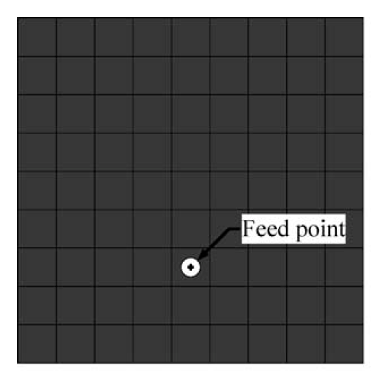
\includegraphics[width=0.3\linewidth]{fig_2_2a.eps}}~~~~~~~~~~~~~~~~~~~~~
  \subfigure[Optimized antenna]{\includegraphics[width=0.3\linewidth]{fig_2_2b.eps}}\\
  \caption [Division of the patch (Gray: metal, White: without metal) (a) Division of patch area (b) optimized patch]{Division of the patch (Gray: metal, White: without metal) (a) Division of patch area (b) optimized patch \cite{optPatch}} \label{fig_2_2}
\end{figure}

An example of a discrete problem is \cite{optPatch}. In this work, binary particle swarm optimization (PSO) technique is used to design a wide-band antenna. In this work, initially, a rectangular patch is taken. The patch is divided into smaller blocks in which the presence and absence of metallization are found using the binary PSO. The original rectangular patch antenna and the final design are shown in Figure \ref{fig_2_2} (a) and (b) respectively. The optimized antenna is basically a slotted rectangular patch antenna in which the position of the slots is obtained algorithmically. The final design has an irregular geometry. The frequency responses of the return loss (S11) parameter of the antenna before and after optimization are shown in Figure \ref{fig_2_3}.

\begin{figure}
  \centering
  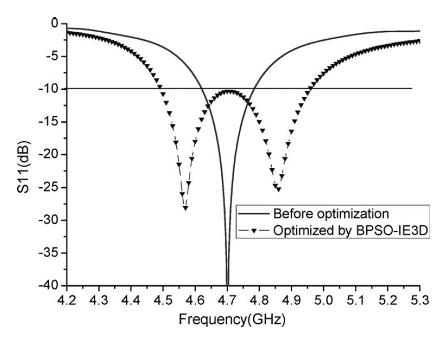
\includegraphics[width=0.3\linewidth]{fig_2_3.eps}\\
  \caption [Computed S11 curves versus frequency]{Computed S11 curves versus frequency. \cite{patch_miniaturize_ga}} \label{fig_2_3}
\end{figure}

In \cite{freqReconfCogn} a similar approach is presented using GA for designing an antenna for cognitive ratio application. In this work, the optimization is applied to find the slot shape and the switches locations in the ground plane of monopole antennas for adjustment of the bandwidth. Here, the switches in the ground plane help in exciting the antenna at different modes. Each mode has its own resonance frequency. Hence, using the switch the resonant frequency of the antenna can be tuned. By using an optimum number of switches, the frequency tuning can be performed by adjusting the minimum possible number of switches without compromising the performance of the antenna.

\subsection{Array Synthesis Problems}
The three crucial conditions for a linear array to meet are \cite{arraySynth1}:
\begin{itemize}
\item \textbf{Gain maximization in the desired direction:} Gain maximization refers to maximizing the far field gain of the antenna along the desired direction in the polar coordinate system defined by azimuth angle ($\phi$), and elevation angle ($\theta$).
\item \textbf{Side-lobe level (SLL) reduction:} SLL reduction refers to suppression of the gain of the antenna array in all directions except the direction of the maximum gain.
\item \textbf{Impedance matching:} In an array, each element is excited individually by a microstrip line in the feeding network. The feed line usually follows a phase shifter or a switch. The objective of the impedance matching problem in array synthesis is to make sure that the complex impedance of each element of the array is matched with the corresponding feed line for each operating mode of the array. If the impedances are not properly matched in an array, the radiation efficiency will be poor.
\end{itemize}

In \cite{arraySynth1}, Z. D. Zaharis et al. proposed a soft-computational approach to design an array that meets all these conditions. In this work, Boolean Particle Swarm Optimization (PSO) technique is used. A large number of evolutionary approaches have been explored worldwide by researchers to design arrays with significant SLL reduction. In \cite{arraySynth2}, the side lobe level of a time modulated linear array is suppressed using non-dominated sorting genetic algorithm II (NSGA-II). Here, the array factor (AF) of the linear array is mathematically represented in terms of Fourier series. The static excitation and the "switch on" time are optimized using the NSGA-II algorithm to minimize the SLL of the array. In \cite{arraySynth3} a new optimization algorithm known as Teaching Learning Based Optimization (TLBO) technique is applied for SLL reduction in SLL. Here also, the excitation parameters are optimized for a linear array to reduce SLL. SLL reduction problem is addressed for both linear as well as circular arrays in \cite{arraySynth4} using a hybrid optimization technique called cuckoo search-chicken swarm optimization (CSCSO). CSCSO combines cuckoo search (CS) which is a global search algorithm and chicken swarm optimization (CSO) which introduce a hierarchy mechanism.

In \cite{compCAD4Arry}, the authors have compared GA, PSO, and DE for the design of a scannable circular array. The designed circular array has a full 360 degree scan at steps of 30 degree. In this work also, optimization techniques are used to calculate the excitation parameters of each element of the array so that gain is maximized along a given direction and SLL is minimized. It is observed from the experimental results presented in \cite{compCAD4Arry} that all the three algorithms yield better performance compared to the conventional case in terms of gain maximization and SLL reduction. However, the results from the different methods are not the same; this is mainly because the algorithms do not guarantee convergence to the global optimum in finite time.

\subsection{Array Thinning Problems}
Thinning of antenna arrays involves the removal (turning off) of some elements in the antenna array so as to maintain radiation properties similar to that of the fully populated array, but using a lower number of elements. Array thinning is a technique in which the spacing between the elements is not uniform. Thinning a large array helps in further reducing its SLL and also reducing the number of antennas in the array and thereby substantially cut down the cost. In most of the cases, analytical approaches are not cost-effective for array thinning problems and therefore soft-computational approaches are most widely used.

In \cite{arrayThin1}, a thinned concentric planar circular antenna array of isotropic elements is designed to generate a pencil beam in the vertical plane with reduced side lobe level and increasing number of switched off elements using an improved variant of DE, called Differential Evolution with Global and Local neighborhoods (DEGL). A new optimization algorithm called the binary spider monkey optimization (SMO) algorithm for designing a thinned concentric circular array is proposed in \cite{arrayThin2}. The array thinning of a concentric circular antenna array is illustrated in Figure \ref{fig_2_4}.

\begin{figure}
  \centering
  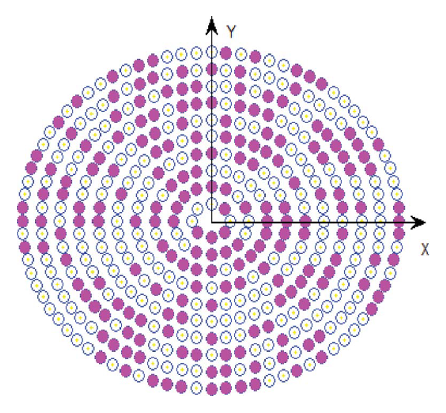
\includegraphics[width=0.35\linewidth]{fig_2_4.eps}\\
  \caption [Isotropic elements (dark shows ON and light as OFF) in ten ring concentric circular antenna array]{440 isotropic elements (dark shows ON and light as OFF) in ten ring concentric circular antenna array. \cite{arrayThin2}} \label{fig_2_4}
\end{figure}

Binary butterfly mating optimization (BBMO) algorithm along with a subarray strategy for thinning of antenna array is proposed in \cite{arrayThin3}. Here, the subarray strategy is dividing the linear array into two parts, one part with a fixed number of element turned on in the middle of the array and the rest elements on the edge of array composing another subarray. In order to reduce the complexity of the thinning process, BBMO algorithm is used to optimize the element on the edge of an array. The proposed BBMO with subarray strategy is used to synthesize a linear sparse antenna array in order to reduce maximum sidelobe level and at the same time keeping the percentage of thinning equal to or more than the desired level.

\subsection{Evolutionary Design of Metamaterial Structures}
Electromagnetic metamaterials are engineered materials that can yield a negative value of its permittivity ($\epsilon$) or permeability ($\mu$) or both at a frequency band of interest. Traditional metamaterial structures include the split ring resonator (SRR), the complementary split ring resonator (CSRR), electromagnetic band-gap (EBG) structures etc. These structures are either built periodically within a dielectric block or fabricated on the surface of an electromagnetic device. A wide range of research works has reported enhancement of the performance of microstrip antennas, wave-guides and other microwave devices on the use of metamaterial structures.

One of the earliest works that reported the use of evolutionary-based approaches in the design of a metamaterial unit cell is \cite{optMtm}. Here, genetic algorithm is used to design algorithm is used to design a metametarial unit cell with negative value of $\mu$ using the filling element methodology. Here square and hexagonal pixels are considered for the design of the metamaterial unit cell. The evolution of the metamaterial structure in this case is illustrated in Figure \ref{fig_2_5}. A similar work for design of metamaterial unit cell using topology optimization is reported in \cite{lh_mtm}.

\begin{figure}
  \centering
  \includegraphics[width=0.35\linewidth]{fig_2_5.eps}\\
  \caption[The best fitness plotted as a function of generation (top). The unit cells show the best structures (elite) at different generations during the evolution process of the GA (bottom)]{The best fitness plotted as a function of generation (top). The unit cells show the best structures (elite) at different generations during the evolution process of the GA (bottom). \cite{optMtm}} \label{fig_2_5}
\end{figure}

\subsection{Evolutionary Design of Metasurfaces}
Metasurfaces are controllable smart surfaces that have a wide range of applications in the design of antennas and other electromagnetic devices. Metasurfaces were proposed in \cite{metasurface1} as a two-dimensional equivalent of the three-dimensional resonant particle type metamaterials. Later, single metamaterial unit cells, also known as planar metamaterials became popular. In the recent years, planar metamaterial unit cells (such as SRR, CSRR, Mushroom-Type EBG unit cell etc.) have been widely reported in the design of microstrip antennas, filters, phase-shifters etc. However, metasurfaces are nowadays incorporated with arrays to reduce the mutual coupling between elements \cite{metasurface2}. In a metasurface based design of microstrip antenna array, the array is sandwitched between two dielectric substrates. The lower face of the lower substrate has the ground plane and the upper face of the upper substrate has the metasurface. The structure is illustrated in Figure \ref{fig_2_6}.

\begin{figure}
  \centering
  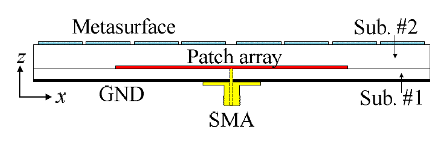
\includegraphics[width=0.6\linewidth]{fig_2_6.eps}\\
  \caption [Cross sectional view of a meta-surface based microstrip antenna array]{Cross sectional view of a meta-surface based microstrip antenna array \cite{metasurface2}} \label{fig_2_6}
\end{figure}

Design of metasurfaces is one of the highly emerging techniques for the improvement of antenna arrays. Genetic algorithm is used for optimization purposes in the design of programmable metasurfaces for active dynamic polarization, scattering and focusing control in \cite{softCompMeta}. In a similar work \cite{uwb_rcs}, a metasurface is designed for reduction of radar cross section (RCS) of an antenna array using polarization convertor and genetic algorithm.

\section{Techniques and Methods for the use of Soft-Computational Approaches in Design of Antennas and Arrays} \label{c2sec_methods}
So far, the various problems in the use of soft-computational approaches for the design of microstrip antennas, arrays and metamaterials are discussed. In this section, the various methods and techniques for the use of soft-computational approaches in the design of antennas and other electromagnetic devices are discussed briefly.

\subsection{Evolutionary Optimization Algorithms}
Evolutionary optimization algorithms are inspired by nature. One of the most commonly used evolutionary algorithm is the genetic algorithm (GA). It mimics the Darwin's theory of natural selection in the evolution of a species. Particle swarm optimization (PSO), another popular algorithm mimics swarm intelligence that include the behavior of ant colonies, bird flocking, animal herding, bacterial growth, fish schooling and microbial intelligence. In recent times, a large number of evolutionary algorithms have been reported enlisted as follows. Differential evolution (DE) is another popular algorithm that is widely used in antenna design. None of these algorithms guarantee global maxima, and based on problem the performance of the algorithms vary \cite{compCAD4Arry}.

In the design of antennas, metamaterial structures and arrays, most of the optimization problems are discrete value problems. The classical GA, PSO, and DE are, on the other hand, designed for continuous value problems. However, there are several variants of these algorithms to address discrete value problems. These methods include binary-coded genetic algorithm (BGA) \cite{optAlgBGAbook, optAlgEMbook}, Binary PSO (BinPSO) \cite{optAlgBPSO}, Boolean PSO \cite{arraySynth1, OptAlgBoolPSO4Ant}, Binary differential evolution \cite{optAlgBinDE, optAlgModBinDE}. In \cite{optAlgDE4AntennaRev}, a detailed analysis of these algorithms is presented along with design of a patch antenna and an array using the novel binary differential evolution (NBDE) algorithm presented in \cite{optAlgModBinDE}.

Apart from these standard evolutionary algorithms, many new evolutionary algorithms have been presented in the recent years. Some of these algorithms, enlisted as follows, are reported in the design of antennas and array design.

\begin{itemize}
\item Teaching learning based optimization (TLBO) algorithm \cite{arraySynth3}
\item Chicken swarm optimization (CSO) algorithm \cite{arraySynth4}
\item Spider monkey optimization (SMO) algorithm \cite{arrayThin1}
\item Binary butterfly mating optimization (BBMO) algorithm \cite{arrayThin2}
\item Cuckoo search (CS) algorithm \cite{CuckooSerach}
\item Invasive Weed Optimization (IWO) \cite{InvasiveWeed}
\end{itemize}

\subsection{Method for Array Synthesis Problems for SLL Reduction and Gain Maximization} \label{c2subsec_sll_methods}
An array comprises of identical antenna elements of known radiation pattern. It is therefore possible to analytically derive the cost function of the optimization problems as in \cite{arraySynth2, arraySynth3, arraySynth4, compCAD4Arry}. The optimization algorithm is used to determine the excitation parameters of each of the elements of the array in order to meet the desired goal of gain maximization or SLL reduction.

In an array, each element is excited separately. In a broad-side array where the main lobe is along a direction perpendicular to the array axis, each element is excited at same phase. In this case, the magnitudes of the excitation parameters are optimized to maximize the gain of the antenna and minimize the SLL. In a scannable array each antenna element is excited at different variable phase. The phase angles are adjusted to tune the direction of the main lobe. In this case, the array factor corresponding to every possible scanning step is optimized by adjusting the magnitudes as well as phase angles of excitation of each antenna element in the array. A computational tool such as MATLAB is sufficient for solving such problems.

When an array synthesis problem includes impedance matching, a full wave model or a surrogate model is required to be incorporated in the system which adds up to the complexity of the problem. These two approaches are discussed in the following sections \ref{c2subsec_thinning} and \ref{c2subsec_tools} respectively.

\subsection{Method for Array Thinning Problems} \label{c2subsec_thinning}
An array thinning problem is initialized with a fully populated array. A binary optimization algorithm is then used to turn off certain elements of the array so that the effect on the overall radiation pattern of the array is insignificant. In such problems also the elements are identical with known far-field radiation patterns. Hence, the cost function of the problem can be derived analytically.

In \cite{arrayThin1, arrayThin2, arrayThin3}, arrays of isotropic antenna elements are used. MATLAB is used in \cite{arrayThin2} and \cite{arrayThin3}. In all these works, the cost function is in terms of SLL reduction. When some elements of a large array are turned off, the SLL of the array increases. Hence, SLL plays a significant role in an array thinning problem. The SLL can be obtained from analytically derived mathematical expressions or from a full wave solver.

\subsection{Interface between Computational Tool and EM Solver} \label{c2subsec_tools}
In order to evaluate the performance of an antenna or an array with high accuracy, a full wave EM solver such as HFSS, CST Studio, IE3D etc. is essential. Optimization algorithms, on the other hand, needs specialized computational tools such as MATLAB. In an evolutionary approach, each generation of the antenna requires independent analysis in order to compute the cost function. In the methods discussed in above Sections \ref{c2subsec_sll_methods} and \ref{c2subsec_thinning}, the cost function is calculated from analytically derived expressions. However, for design of a single antenna element \cite{patch_miniaturize_ga, optPatch, freqReconfCogn} or an array synthesis problem involving impedance matching \cite{arraySynth1}, such an approach is not reliable. It is therefore necessary to integrate the computational tool and the EM solver, so that the antenna is iteratively designed and evaluated with high accuracy.

The flow diagram of genetic algorithm based design of a rectangular patch antenna reported in \cite{patch_miniaturize_ga} is shown in Figure 7. It is observed from the figure that the antenna is modeled in CST studio, which is a full-wave EM solver. The genetic algorithm is implemented in MATLAB. Such arrangement helps in accurate evaluation of the antenna for best performance.

\begin{figure}
  \centering
  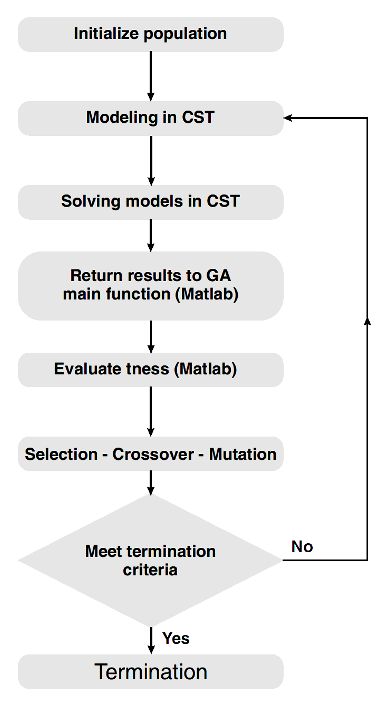
\includegraphics[width=0.4\linewidth]{fig_2_7.eps}\\
  \caption[A block diagram of genetic algorithm function used in this design]{A block diagram of genetic algorithm function used in this design \cite{patch_miniaturize_ga}} \label{fig_2_7}
\end{figure}

In \cite{optPatch}, the EM solver used is IE3D. Here, the design parameters are written to a file which is read by the IE3D solver. After simulation, the IE3D solver writes the data to another file which is read from MATLAB for computation of the cost function and the design parameters for the next iteration. A custom EM solver is used in \cite{arraySynth1} for an array synthesis problem involving impedance matching in a similar approach.

HFSS, another popular EM solver tool, supports a script interface. Any antenna can be designed and analyzed by writing a script. This script interface can be used for the designing of an antenna in MATLAB and exporting it to HFSS. In the script, HFSS may be instructed to store the result in a specified file which can later be read from MATLAB to obtain the simulation results.

\subsection{Surrogate Model Assisted Optimization}
A full-wave EM simulation involves a huge set of computations and hence such simulations are often time consuming. This significantly limits the efficiency of evolutionary approaches for the design of antennas. A solution to this problem is the introduction of a surrogate model. In \cite{antSurrD01}, a surrogate model assisted evolutionary algorithm (SAEA) is proposed. Here, a surrogate model is a Gaussian process model of the actual full-wave simulations. Surrogate modeling methods include Gaussian process or Kriging, response surface methods, artificial neural networks (ANN), support vector machines and radial basis function models. A surrogate model is derived from actual full-wave simulation. At every iteration of the evolutionary algorithm, the cost function is evaluated from the surrogate model instead of the actual full-wave simulation. This significantly enhances the efficiency of the optimization process.

Surrogate models based approaches are being explored for various antenna design problems in the recent years. In \cite{surrMTM01}, a surrogate model assisted optimization technique for metamaterial devices is proposed. Surrogate models are explored in \cite{antSurrConstMO} for constrained, multi-objective antenna design problems.

\section{Conclusion}
The various problems in soft-computational approaches for designing of antennas and arrays are summarized. Soft-computational approaches have a number of advantages over the traditional approaches for antenna design. Evolutionary-based algorithms are basically search algorithms which can find an optimized solution in the solution space. Soft-computational tools can be helpful if the search space is large. Techniques such as surrogate model helps in reducing computation time; however, synthesis of the surrogate model is another area of research.

\chapter{Simulation-Driven Optimization of Slot Antenna using Genetic Algorithm}
\label{chap:chap3}
\section{Introduction}\label{c3sec_intro}
Microstrip antennas were the first printed patch antennas. The concept of microstrip antennas was first proposed in 1953 by G. A. Deschamps et al. \cite{mpa00}. Microstrip antennas and arrays were practically fabricated in the 1970s in several contemporary works such as \cite{mpa02} and \cite{txmPhasedArray}. The design trends until the beginning of the 1980s were covered in a survey work by K. R. Karver et al \cite{mpaSurvTech}. This review gives significant insights into the design trends until that period. The number of works related to microstrip antennas increased exponentially over the years after 1980 \cite{mpaHist01}. The designing of microstrip antenna arrays was another trend that evolved almost simultaneously. At that time, microstrip antennas were known for their disadvantages of low gain and bandwidth. This may be a reason why many researchers considered the design of compact, rigid and planar arrays using microstrip antennas to enhance the gain. In 1974, a phased array of microstrip antenna elements was proposed by R. F. Munson \cite{txmPhasedArray}.

In the initial phase, most of the works on microstrip antennas were related to feeding mechanisms. These works were based on some simplifying approximations for making them computationally simple. These models provide useful information regarding impedance, radiation patterns, efficiency and bandwidth of the antennas \cite{mpaReview1992}. The two most commonly used feeding mechanisms for microstrip antennas are the microstrip line feed and the coaxial feed. These two techniques are widely in practice since the 1970s.

Between the mid-1970s and early 1980s, for the first time, several research works reported the design and modeling of microstrip antennas. The transmission line model and the cavity model were formulated during this period \cite{handbook}. The generalized transmission line model and the generalized cavity model were proposed in the the 1980s, which extended the transmission line model and the cavity model respectively to include microstrip antennas with more complex shapes \cite{handbook}. Finally, with the availability of modern computers, full-wave electromagnetic solvers were created. By the 1990s there were commercially available full-wave electromagnetic solvers. This led to a remarkable increase in the volume of research publications in the field of antenna design. Antennas with highly complex geometrical structures can be easily designed and simulated using software applications such as HFSS{\circledR}, CST{\circledR}, etc \cite{practGuide3D}. Antennas of various sizes and shapes were designed during this period \cite{smallPatch0, BandSize0, HPatch1, uslot1, dualBandCircPol, dualBandWLAN, fractal1, slottedUWB, bandnotchCSRR1, bandnotchEBG1, SlottedPatchModel, spiralSlotGnd, GndSRRPatch}. The analytical modeling and parameterizations of antennas, on the other hand, became less popular. The few analytical works published in this period were primarily concerned about developing an overall understanding of the antenna rather than formulating a design methodology. The designs are mostly validated from simulation and measurement results.

Equivalent circuit modeling of antennas is a more recent approach to antenna modeling. In this approach, the antenna is modeled as an RLC network \cite{rectEqCkt, Broadband_EqCkt, UwbEqCktMethod, UwbPmaEqCkt1, UwbPmaEqCkt2, UwbPmaEqCkt3, UwbPmaEqCkt4, UwbNotchEqCkt}. The representation of the input impedance is a challenging task in equivalent circuit modeling. Results obtained from a high-fidelity full-wave model are often used for setting and tuning the parameters of an equivalent circuit model.

In recent years, soft-computational optimization algorithms are becoming popular for the design of microstrip antennas and arrays \cite{UwbPmaGaFdtd, cadNASA, compCAD4Arry, antSurrD01, surrMTM01, antSurrConstMO}. Soft-computational designs involve iterative adjustment of the geometrical parameters of an antenna using a soft-computational optimization algorithm to obtain optimized values of the performance parameters such as resonant frequency, gain, bandwidth, etc. The process requires the computation of the electromagnetic parameters of an antenna at each iteration of the optimization algorithm. The full-wave methods are computationally very expensive and time consuming for iterative computation. Surrogate models have emerged as a solution to this problem.

In \cite{patch_miniaturize_ga}, the dimensions of a rectangular patch antenna are optimized using genetic algorithm (GA). Five physical dimensions of the antenna are tuned algorithmically to optimize the antenna. This is a 5-dimensional continuous problem. Here, the antenna is simulated in CST studio in order to calculate the cost function and the genetic algorithm is implemented in MATLAB.

In \cite{freqReconfCogn} a similar approach is presented using GA for designing an antenna for cognitive ratio application. In this work, the shapes of the slots and the locations of the switches in the ground plane are optimized for adjustment of the bandwidth. Here, the switches in the ground plane help in exciting the antenna at different modes. Each mode has its own resonance frequency. The antenna can be tuned to resonate at different frequencies with the help of the switches. The optimization problem was aimed to minimize the number of switches so that the same dynamic range of the resonant frequency of the antenna can be obtained with a minimum number of tunable parameters.

One of the earliest works that reported the use of evolutionary-based approaches in the design of a metamaterial unit cell is \cite{optMtm}. Here, genetic algorithm is used to design a metametarial unit cell with negative value of $\mu$. This is a discrete problem where the final structure is constructed by iteratively filling the area with small structural elements. A similar work for design of metamaterial unit cell using topology optimization is reported in \cite{lh_mtm}.

Soft-computational algorithms are also widely used for the design of arrays. Array optimization includes a wide range of applications such as array synthesis \cite{arraySynth1, arrayThin1}, array optimization \cite{arraySynth3}, side lobe level (SLL) reduction \cite{arraySynth2, arraySynth4}, etc. In \cite{compCAD4Arry}, a comparison of genetic algorithm (GA), particle swarm optimization (PSO), and differential evolution (DE) is presented in terms of their application in the optimization of planar arrays.

Traditionally, computational tools such as Matlab or Python are used for implementing optimization algorithms, whereas antennas are simulated with commercially available full-wave solvers such as AEDT (or HFSS), CST studio, etc. Setting up different software applications together in order to perform the optimization is a computationally intensive task. AEDT provides an Iron-Python script interface which can be used for automating certain simulation tasks. It is a limited implementation of Python that lacks support for many packages, crucial for implementing computationally intensive algorithms. Here, the genetic algorithm is implemented with Iron-Python that functions within AEDT and does not need any external libraries to be installed.

The remaining part of this chapter are arranged as follows. Section \ref{c3sec-prop-alg} contains the details of the proposed method for implementing the genetic algorithm in AEDT. Section \ref{c3sec-exp-details} covers the details of the experiment formulated to test the proposed approach. The experimental results are discussed in Section \ref{c3sec_expt-res}. Finally, the chapter is concluded in Section \ref{c3sec_concl}.

\section{Details of the Proposed Algorithm} \label{c3sec-prop-alg}
\begin{figure}
  \centering
  \includegraphics[width=0.6\linewidth]{bc-flowchart.eps}\\
  \caption{Flowchart of the implementation of genetic algorithm in AEDT}\label{fig1}
\end{figure}
Genetic algorithm is a bio-inspired optimization algorithm. It is a global-search algorithm that mimics the principle of natural selection to arrive at a global maximum point in the search space. The algorithm iteratively generates samples to minimize the error, given by a cost function. This section provides the details of how the cost function is formulated in an antenna optimization problem followed by the details of the genetic algorithm and its various terms in the context of antenna optimization.

\subsection{Cost Function for Antenna Optimization}
In case of antenna optimization, the cost function is derived from the performance parameters of the antenna such as resonant frequency, bandwidth, far-field gain etc. The variables to be optimized are the physical dimensions of the antenna such as length, width, position of the feed etc. The cost function yields the difference between the actual and the desired performance of the antenna. For example, if the design goal is to obtain resonance at a particular frequency, the cost function will be:
\begin{equation}
E = \left|f_{\textrm{target}}-f_{\textrm{obtained}}\right|
\end{equation}

If the desired antenna has two resonant frequencies $f_1$ and $f_2$, the goal is to minimize the return loss ($S_{11}$) parameter at these two frequencies. Accordingly, the cost function may be formulated as follows.
\begin{equation}
E = \max\left(S_{11}(f_1), S_{11}(f_2)\right)
\end{equation}
If the goal is to maximize the far-field gain, the cost function will be
\begin{equation}
E = \left|G_{\textrm{target}}-G_{\textrm{obtained}}\right|
\end{equation}

In order to calculate the error using the cost function, it is important to evaluate the performance of the antenna corresponding to the generated set of dimensions of the antenna. Full-wave electromagnetic solvers are the most reliable tools for this purpose. Fig. \ref{fig1} shows the flowchart of the technique used for implementing the genetic algorithm for optimizing antennas with AEDT. The dimensions are initialized arbitrarily. The genetic algorithm then iteratively updates the dimensions to minimize the error given by the cost function. The cost function depends on the design goals.

\subsection{Genetic Algorithm for Antenna Design}
The term ``Genetic algorithms'' refer to a number of implementations of an optimization algorithm inspired by the law of natural selection. Many of these techniques are discussed in \cite{gaBook}. In the present work, the implementation of genetic algorithm is inspired by the algorithm reported in \cite{gaImpl}. This section breaks down the genetic algorithm terminologies in a way to fit into the context of antenna optimization.

Like any other soft-computing technique, genetic algorithm also has some hyper-parameters that must be pre-defined for the given problem. The hyper-parameters of a genetic algorithm includes the DNA size, population size and the number of generations. The dimensionality of the optimization problem is represented by the DNA size. It is equal to the number of dimensions that are to be optimized. The maximum number of iterations to be performed before terminating the optimization process is represented by the number of generations.

Most of the terminologies used in genetic algorithm are directly borrowed from biology. These are generalized terms and it is important to understand their meanings to be able to relate these terms with the optimization problem that need to be solved. Some terminologies of genetic algorithm and their interpretation in terms of antenna optimization are discussed as follows.

\begin{itemize}
\item \textbf{Selection of the initial population:} The initial population is an array of random values of the dimensions of the antenna. Each element of the array is another array of the size equal to the DNA size. For example, if four physical dimensions of the antenna are to be optimized using genetic algorithm, the initial population will be $N$ arrays each having four elements. Each array is called a chromosome. A chromosome, thus is a possible solution to the optimization problem. Each element of a chromosome is called a DNA and it corresponds to a particular physical dimension of the antenna that needs to be optimized.
\item \textbf{Assigning Weights to the Chromosome:} The fitness of a chromosome is inversely related to its cost function. If the cost function of a particular set of dimensions is high, it has a low fitness. Thus, for every chromosome, the full-wave simulation is to be executed in order to obtain its electromagnetic parameters. This is the reason why the genetic algorithm has a very high time consuming when used to solve an antenna optimization problem. If the cost function of a particular solution is $c$, its fitness value is considered as $1/c$. This fitness value is assigned as its weight.
\item \textbf{Weighted Selection:} This is the step where chromosomes are selected for the next generation (iteration). Two sets of dimensions are selected that has the maximum fitness value. If the fitness is greater than a threshold, the optimization process is terminated and the available solution with the maximum fitness is the optimal solution to the problem. If the fitness of all the chromosomes is less than the threshold, a chromosome with the maximum fitness is used to obtain the next generation. In case of antenna optimization, a set of dimensions is selected in this step that has the minimum cost function in terms of the given design criteria.
\item \textbf{Mutation:} Mutation is the process by which the next generation is obtained from the chromosome selected in the previous step. A small random number is added to each physical dimension (DNA) of the chromosome in order to obtain the next generation. In other words, each physical dimension of the antenna leading to the minimum value of the cost function is slightly distorted to obtain the next generation.
\item \textbf{Crossover:} In some optimization problems, the next generation is obtained by combining a pair of two chromosomes with minimum loss. In this case, some DNAs from one chromosome and some DNAs from the other chromosomes are interchanged at different positions. This technique, however, is not always suitable for antenna optimization. Each dimension of the antenna has a particular range. Hence, two DNAs corresponding to two different physical dimensions cannot be interchanged to perform a crossover. That is why crossover is not performed in the present work.
\end{itemize}

\begin{figure}[h]
\centering
\includegraphics[width=0.9\linewidth]{bc-ga-flow.eps}
\caption{Flow diagram of the implementation of genetic algorithm for antenna optimization.}\label{ga-flow}
\end{figure}

The steps discussed are presented as a flowchart in the context of antenna design in Fig. \ref{ga-flow}. Here, all terminologies of genetic algorithm are replaced by antenna design terminologies in order to make the process easily relatable to the context of antenna design. Crossover is not performed in this case and the next generation is obtained from the set of dimensions with the minimum value of the loss function through the process of mutation by adding some small random numbers.

\section{Experimental Details} \label{c3sec-exp-details}
This section covers the details of an experimental evaluation of genetic algorithm for optimizing a printed antenna. The method discussed in the Section \ref{c3sec-prop-alg} is used here to optimize an H-shaped slot antenna. Slot antennas are printed antennas. Unlike microstrip antennas, the slot antenna has a slotted section etched from the ground plane. Slot antennas are excited with a microstrip line present at the opposite face of the PCB. Coplanar wave-guide (CPW) may also be used for exciting a slot antenna.

A dual-band H-shaped slot antenna is designed that resonates at 2.4 GHz and 3.6 GHz. The top view and the bottom view of the proposed antenna are shown in Fig. \ref{h-shaped-topology}. The antenna has several dimensions. The size of the search space increases exponentially increases with the dimensionality and therefore the number of iterations required to obtain the optimized dimensions of the antenna also become very large. A full-wave electromagnetic solver may take several minutes to simulate an antenna and generate the performance parameters. The actual computation time depends on the size and complexity of the antenna.

Here, the antenna is designed through experimental method and the genetic algorithm is used only for tuning the position of the feed point. The other dimensions of the antenna are shown in Table \ref{tab-h-dim}. Glass fiber (FR4-Epoxy) substrate is used for fabrication of the antenna that has a relative permittivity, ($\epsilon_r$), of 4.4.
\begin{figure}[h]
\centering
\subfigure[]{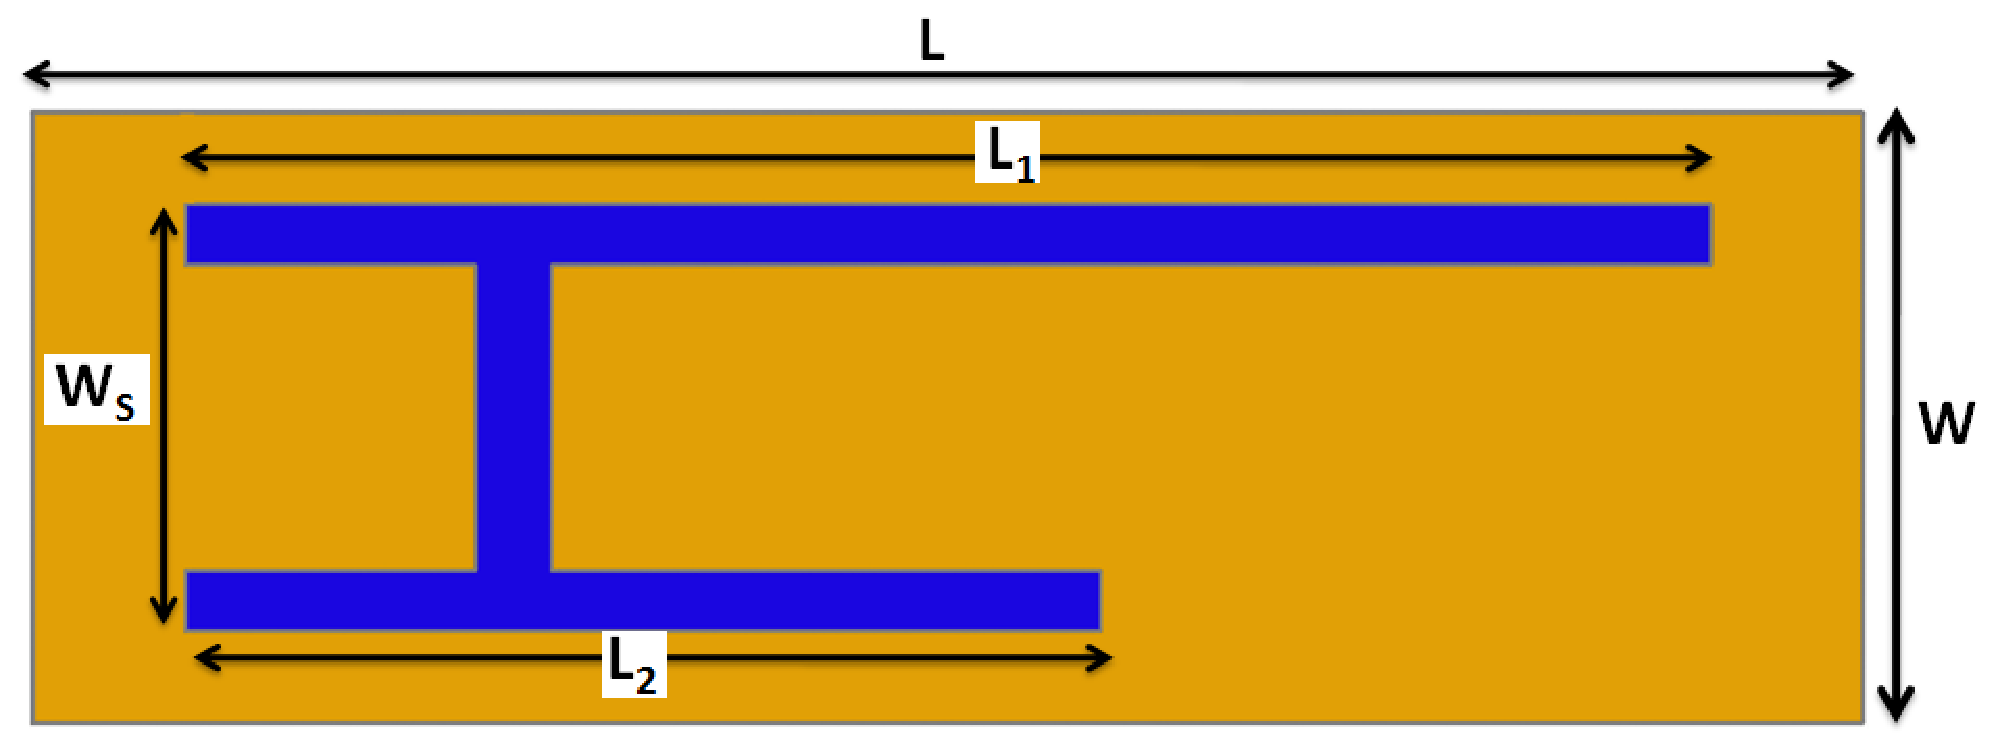
\includegraphics[width=0.7\linewidth]{bc-ant_top.eps}}\\
\subfigure[]{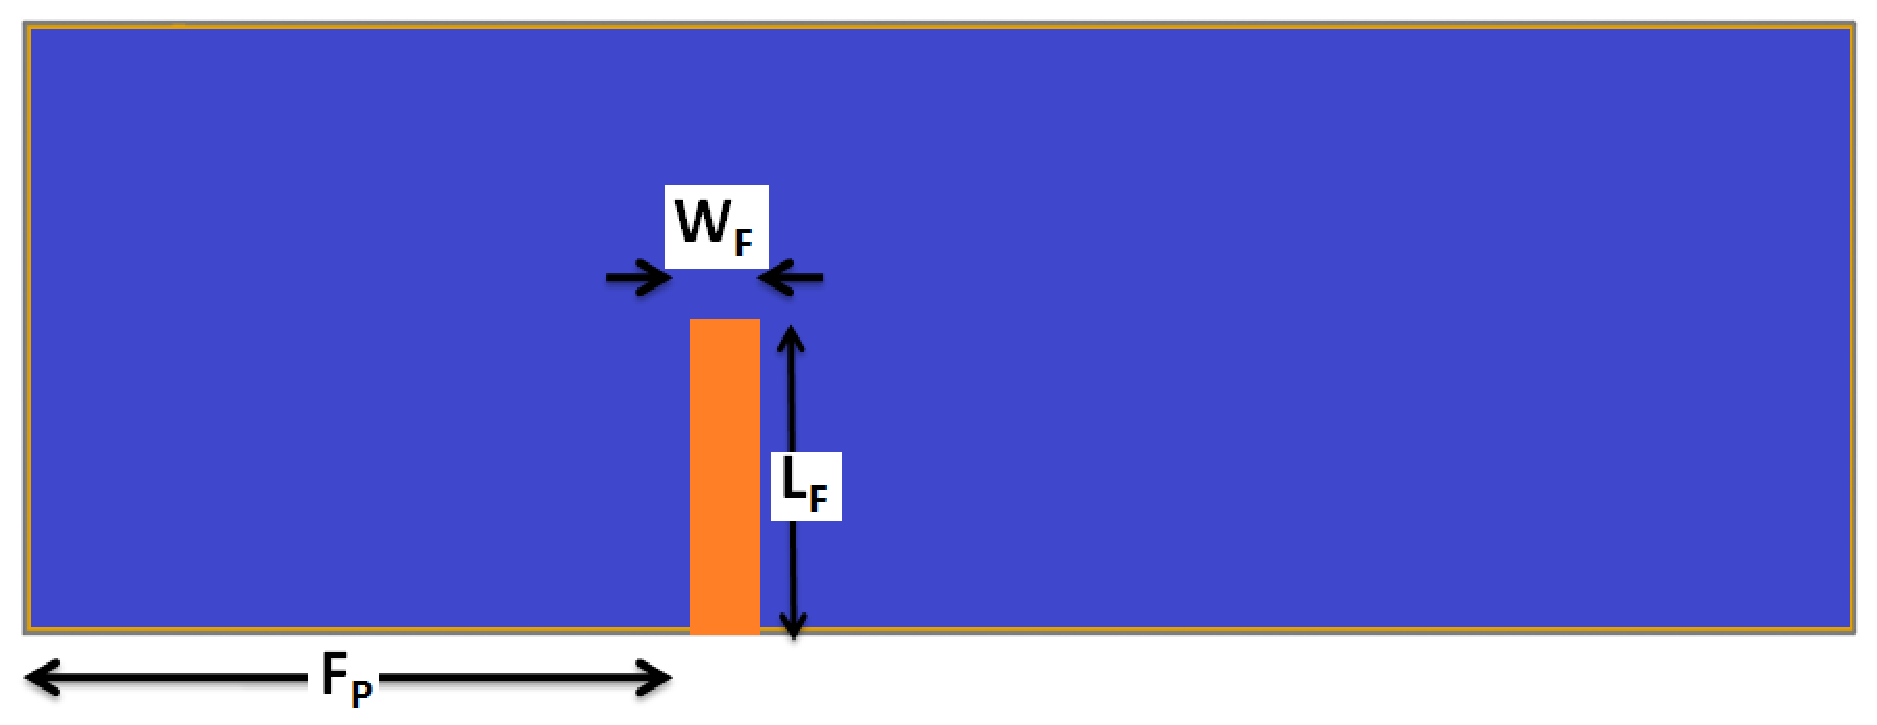
\includegraphics[width=0.7\linewidth]{bc-ant_back.eps}}\\
\caption{(a) Top view and (b) Bottom view of the example antenna}\label{h-shaped-topology}
\end{figure}

\begin{table}[h]
\centering
\caption{Dimensions of the test antenna} \label{tab-h-dim}
\label{tab:my-table}
\resizebox{0.5\textwidth}{!}{%
\begin{tabular}{|l|c|}
\hline
\textbf{Dimension} & \textbf{Value (mm)} \\ \hline
Length of the substrate ($L$) & 60 \\ \hline
Width of the substrate ($W$) & 20 \\ \hline
Length $L_1$ of the H-slot & 50 \\ \hline
Length $L_2$ of the H-slot & 30 \\ \hline
Width of the H-slot($W_S$) & 14 \\ \hline
\end{tabular}}
\end{table}

Optimizing the feed position of an antenna is an one-dimensional problem, that is, its DNA size is one. Since antenna simulation is a time-consuming task, the population size is kept small. In this case, the population size is five. The maximum number of generations is kept 50. The antenna is optimized to obtain its resonant frequencies at 2.4 GHz and 3.6 GHz. Hence, the cost function is derived as shown in Equation \ref{dual_cost}:

\begin{equation}\label{dual_cost}
\text{error}=\left|f_{r1}-2.4\times10^9\right|+\left|f_{r2}-3.6\times10^9\right|
\end{equation}

Here, $f_{r1}$ and $f_{r2}$ respectively are the first and the second resonant frequencies of the antenna. The resonant frequencies are obtained at the local minimum points of the S11 parameter plot. The python script saves the S11 parameter plot as a CSV file and then reads the file to find the minimum points of the S11 parameter.

The time required for running one simulation depends on a many of factors. If the antenna has a complex or circular geometry, the computation time is high. If the geometry of the antenna is simple, the computation time is relatively low. The computation time also depends on the frequency range over which the simulation is performed. The final antenna has a feed potion 35 mm.

The script interface of AEDT enables an user to create elements, change variables, run simulations and export the results to files. It is not possible to access the simulation results directly using the scripts. Further, the iron-python interface of AEDT lacks support for many python packages, such as SciPy, NumPy, Random, etc. that are crucial for implementing algorithms involving mathematical operations.

These problems are addressed by writing own programs for micro-tasks such as generating random numbers, dividing mathematical expressions into smaller arithmetic blocks, etc. In order to obtain the s11 parameters for evaluating the cost function,, the results are first exported to a CSV file and then read programmatically and parsed the data.

\section{Experimental Results} \label{c3sec_expt-res}
This section provides the details of the optimized antenna. The optimized H-shaped slot antenna is fabricated on a copper-FR4 PCB board. The fabricated antenna is shown in Fig. \ref{h-shaped-fab}. The performance of the antenna is evaluated from the return loss parameter (S11) plot and the far field radiation patter. In Fig. \ref{fig-s11-opt}, the simulated and the measured $S_{11}$ parameter plot of the antenna are shown. It is observed that the optimized dual-band antenna has resonant frequencies at 2.4 GHz and 3.6 GHz. The radiation patterns of the antenna at the two resonant frequencies are shown in Fig. \ref{fig-pattern}.

\begin{figure}
\centering
\subfigure[]{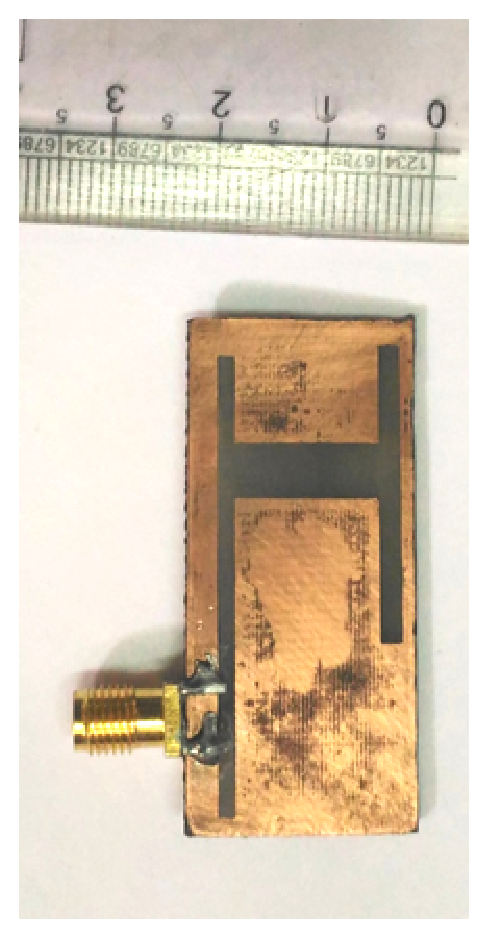
\includegraphics[width=0.3\linewidth]{bc-fab-front-h-slot.eps}}~~~
\subfigure[]{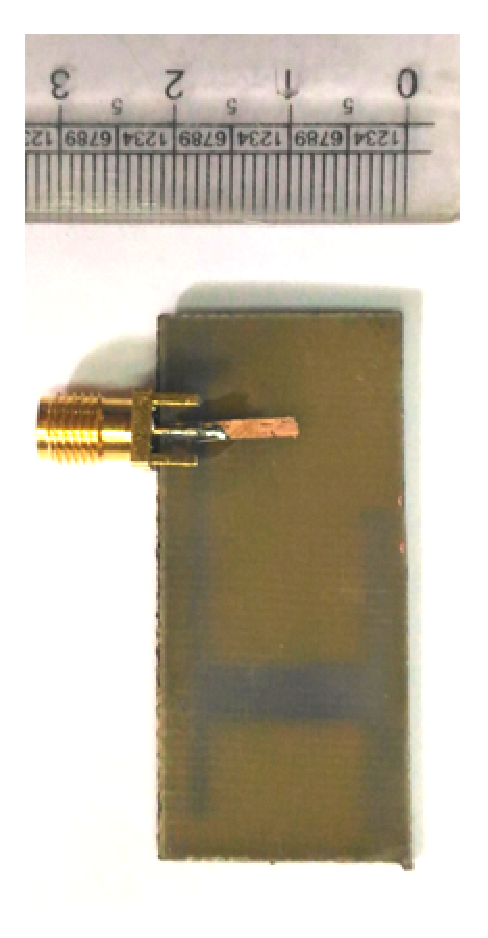
\includegraphics[width=0.3\linewidth]{bc-fab-back-h-slot.eps}}\\
\caption{(a) Top view and (b) Bottom view of the fabricated antenna}\label{h-shaped-fab}
\end{figure}

From Fig. \ref{fig-s11-opt}, it is observed that the antenna resonates at 2.4 GHz and 3.6 GHz. The simulated and the measured result shows a good agreement. This is possible because of the full-wave simulation used for computing the cost function. The full-wave simulation provides very high accuracy. This ensures minimum deviation between the optimized antenna for real-world application. The S11 parameter plot further shows that the antenna is useful for the ISM bands of 2.4 GHz and 3.6 GHz. The bandwidth of the antenna is about 200 MHz at the 2.4 GHz and about 700 MHz at the 3.6 GHz.

\begin{figure}
\centering
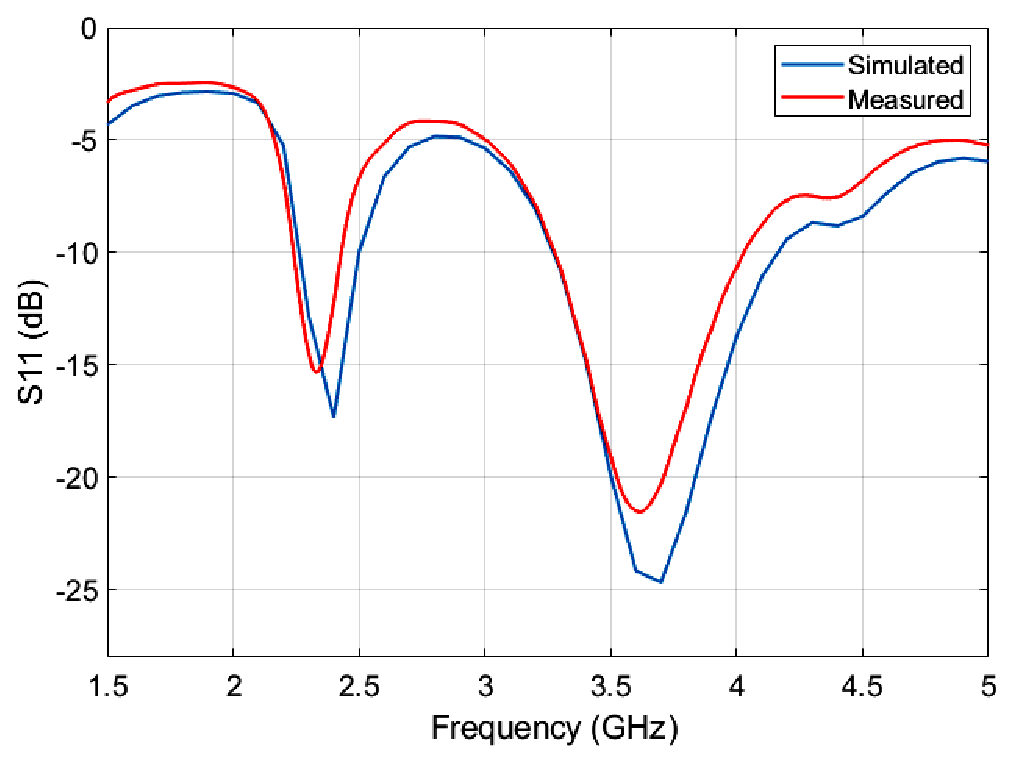
\includegraphics[width=0.7\linewidth]{bc-s11_res.eps}\\
\caption{Simulated and measured $S_{11}$ parameter plot of the optimized antenna}\label{fig-s11-opt}
\end{figure}

The radiation pattern of the antenna was not optimized. It is observed that the antenna has a far-field gain of 2 dBi in the direction of the major lobe ($\theta=0$) for both 2.4 GHz and 3.6 GHz. Thus, the antenna has almost the same sensitivity in this direction at both of its resonant frequency. However, the resonant frequency at 3.6 GHz is clearly is a higher order mode of the antenna and hence its radiation pattern has more than one major lobe.

\begin{figure}[h]
\centering
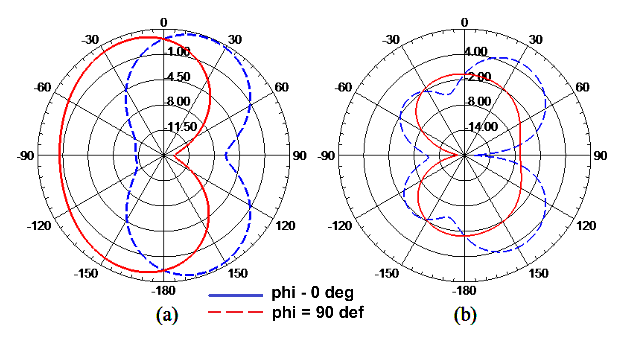
\includegraphics[width=0.7\linewidth]{bc-patterns.eps}\\
\caption{Far field radiation pattern of the proposed antenna at (a) 2.4 GHz and (b) 3.6 GHz}\label{fig-pattern}
\end{figure}

From the experimental results discussed, it is observed that the optimization algorithm is capable of meeting design criteria as specified in the cost function. However, the optimization algorithm cannot ensure that the other parameters of the antenna are also within conventionally acceptable limits. Constructing more complex cost functions may help in meeting multiple design goals. The high time requirement of full-wave techniques is the biggest drawback of this approach. To meet multiple design goals, it is important to tune multiple physical dimensions of the antenna. This leads to an exponential increase of the number of simulations to be performed.

\section{Conclusion}\label{c3sec_concl}
Genetic algorithm is one of the most popular bio-inspired optimization techniques. It has a wide range of application in various fields. There are many different implementations of this algorithm for various problems. An implementation of the genetic algorithm is presented for optimization of printed antenna with Ansys AEDT. The feed position of a H-shaped slot antenna is optimized with the proposed technique. The full-wave electromagnetic solver is used in each iteration of the optimization loop to calculate the cost function.

This approach guarantees a minimum difference between simulation and measurement results. However, the approach does not guarantee good performance of other electromagnetic parameters that may be desirable in a given case. Further, full-wave electromagnetic solvers require more time and computational resources as compared to other approximation based approaches. It is therefore not always feasible to optimize multiple dimensions of an antenna with this approach. The number of iterations required increases with the number of dimensions to be optimized. A time required for the optimization process in this case may range from several hours to several days depending upon the complexity of the design and the capacity of the computational hardware. However, the time required in this case is less compared to the optimetric tool that comes in-built with AEDT. The optimetric tool simulates the antenna for all possible values of the design parameters without any feedback loop. The feedback loop in genetic algorithm helps in significantly reducing the number of simulations required.

Here, the genetic algorithm is implemented using the Iron-Python script interface available with AEDT. This is a very minimal implementation of Python and lacks the support of various python packages that are vital for numerical computations of any kind. This  adds to the challenges in implementing soft-computing techniques such as genetic algorithm. There are other approaches where a more powerful computational tools such as Matlab is interfaced with the AEDT for better performance. The proposed approach requires less computational resources at the cost of an increased complexity of implementation. It can possibly speed up the optimization process in certain cases.

\chapter{Design of a Dual-Band Multilayer Antenna and its Equivalent Circuit Modeling with Vector-Fitting and Genetic Algorithm}
\label{chap:chap4}
\section{Introduction}\label{intro}
Antennas can be broadly classified as directional antennas and omnidirectional antennas. Conventional microstrip antennas, because of its ground plane, provides a directional radiation pattern \cite{handbook}. A printed monopole, on the contrary, provides an omnidirectional radiation pattern \cite{pma_stripline, pma_dualband}. Printed monopoles are variants of microstrip antenna which is characterized by the absence of a ground plane below the patch. A printed monopole excited by a microstrip line has a ground plane below the feed line \cite{pma_stripline}. Printed monopoles are low profile antennas for high gain and high bandwidth with an omnidirectional radiation pattern\cite{PMA01}.

A number of techniques have been explored for building and improving microstrip antennas in the last few decades. One of these techniques is to build multi-layer structures of printed antennas. Multi-layer printed antennas are known for providing wide bandwidth \cite{ML_WideBand01}, resonance at more than one band \cite{ML_DualBand01, ML_DualBand02}, and high gain \cite{ML_high_gain_parasitic_slot}.

Recent trends show that 5G standards are mostly set around directional communication techniques where spatial diversity is utilized to its maximum potential \cite{5G_surv1, 5G_surv2}. Low cost deployment of IoT, on the other hand, relies on traditional ISM band communication with omnidirectional antennas \cite{iot-ant1,iot-ant2,iot-ant3}. When a 5G back-haul link is to be provided to an IoT network in star topology, the traditional approach is to use separate antennas at the hub for 2.4 GHz ISM band and 5G. This adds up to the size and complexity of the system.

In this paper, a multi-layer, dual-band antenna is presented which provides an omnidirectional radiation pattern at the 2.4 GHz ISM band and a high-gain, directional radiation pattern at a wide band ranging from 3.6 GHz to 4.2 GHz. The band between 3.6 GHz to 4.2 GHz is important because it covers most of the sub-bands of the 5G C-band \cite{5G_tutorial, 5G_standards}. The proposed antenna can be used at the hub of an IoT network operating at the 2.4 GHz ISM band for providing a 5G back-haul link. The hub is usually a fixed device which can be installed in such a way that it has a directional link with the nearest 5G base station. An equivalent circuit model of the antenna is derived to explain the behavior of the antenna. The circuit parameters are obtained with vector-fitting and also with genetic algorithm.

The printed monopole as well as the superstrate affects the resonant frequencies of the antenna. Hence, each parameter can be tuned to optimize its overall performance. The design details of the proposed antenna along with the formulation of the equivalent circuit model is discussed in Section \ref{sec:design}. Section \ref{sec:analysis} presents an analysis of the antenna with the equivalent circuit model. The simulation and measurement results of the antenna are presented in Section \ref{sec:expt_results}. Finally, the communication is concluded in Section \ref{sec:concl}. All full-wave simulation results reported are performed with Ansys Electronic Desktop (AEDT).
\section{Design Details of the Proposed Antenna}\label{sec:design}
The proposed antenna is the hybrid of a printed monopole antenna and a microstrip antenna. The printed monopole antenna has an omnidirectional radiation pattern at the 2.4 GHz ISM band. The microstrip antenna has a directional pattern at the C band. The capacitor represents the physical separation between the two branches. The design details of the antenna and its equivalent circuit model are discussed in this section.

\begin{figure}[t]
\centering
\includegraphics[width=0.5\linewidth]{Fig-aeue_1.eps}
\caption{Schematic of the proposed antenna. (a) Top view (b) Side view}\label{topology}.
\end{figure}

\subsection{Topology of the Proposed Antenna}
The first step in this approach is the design of a single printed monopole with a wide bandwidth. The printed monopole is excited with a microstrip line. When the length of a microstrip line is more, the effect of surface-wave loss and radiation-loss become significant. These losses are more at higher frequencies and are more prominent at points of discontinuity \cite{rad_loss}. A discontinuity is introduced in the feed-line by loading it with a dielectric slab cladded with copper on the top. At the point where this slab is loaded, the effective dielectric constant of the microstrip line experiences a change. This leads to an electromagnetic discontinuity that can cause surface-wave loss and radiation loss in the microstrip line. At lower frequencies, this loss is less and hence most of the power is coupled to the printed monopole resulting in a omnidirectional radiation pattern. At higher frequencies, most of the power is coupled to the metallization above the dielectric slab. This results in a directional radiation pattern at the upper resonant frequency of the antenna. The metallization acts like a proximity coupled microstrip patch antenna.

The topology of the antenna is shown in Fig. \ref{topology}. The dielectric material used for the substrate and the superstrate is FR4 epoxy which has a relative permittivity ($\varepsilon_r$) of 4.4. This thickness of each dielectric slab is $1.5mm$. The values of the physical dimensions of the antenna are shown in Table \ref{table-dims}.
\begin{table}
\centering
\caption{Dimensions of the antenna} \label{table-dims}
\begin{tabular}{|l|r|}
\hline
\textbf{Dimension} & \textbf{Value (mm)} \\ \hline
Length of the substrate, $l$ & 50 \\ \hline
Width of the substrate, $w$ & 50 \\ \hline
Length of the patch, $l_P$ & 20 \\ \hline
Width of the patch, $w_P$ & 20 \\ \hline
Length of the superstrate, $l_S$ & 17 \\ \hline
Width of the superstrate, $w_S$ & 25 \\ \hline
Length of the feed line, $l_F$ & 27 \\ \hline
Width of the feed line, $w_F$ & 2 \\ \hline
Longitudinal spacing between patch and superstrate, $s$ & 2 \\ \hline
Height of the substrate and superstrate, $h$ & 1.5 \\ \hline
\end{tabular}
\end{table}

\subsection{Formulation of the Equivalent Circuit Model of the Antenna}
The antenna with the dimensions shown in Table \ref{table-dims} is fabricated using copper-FR4 epoxy printed circuit board (PCB). The fabricated antenna structure is shown in Fig. \ref{FabEqckt} (a). An equivalent circuit model of the proposed antenna is also derived from the analysis. Fig. \ref{FabEqckt} (b) shows the equivalent circuit along with demarcations showing respective LCR sections for the printed monopole and the superstrate.

The equivalent circuit is derived from the fundamental transmission line theory. Here, the printed monopole patch for its first resonant frequency is modeled as a narrow-band parallel LCR circuit \cite{UwbPmaEqCkt1}. The inductor, $L_p$, and the capacitor, $C_p$ correspond to the printed monopole. The superstrate is represented with the equivalent circuit of a transmission line model with a series inductor, $L_s$, and a shunt capacitor, $C_s$. The capacitor $C_c$ represents the coupling between the printed monopole and the superstrate. The inductance $L_{f}$ and the capacitance $C_{f}$ represent the microstrip line feed used. The two load resistances $R_{Rad1}$ and $R_{Rad2}$ correspond to the radiation resistances of the printed monopole and the superstrate respectively. $R_{\text{in}}$ is the input impedance of the source which is equal to $50~\Omega$.

\begin{figure}
\centering
\subfigure[]{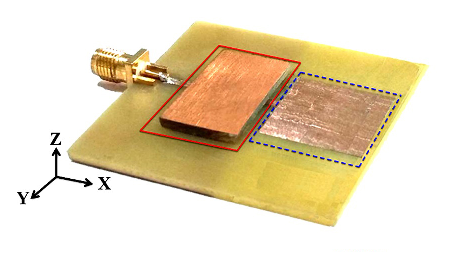
\includegraphics[width=0.4\linewidth]{Fig-aeue_2a.eps}}~~~~
\subfigure[]{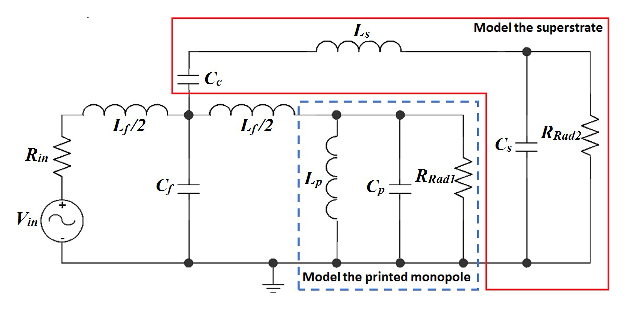
\includegraphics[width=0.6\linewidth]{Fig-aeue_2b.eps}}
\caption{(a) The fabricated antenna and (b) the equivalent circuit model of the antenna along with demarcations showing respective LCR sections for the printed monopole and the superstrate.}\label{FabEqckt}
\end{figure}

The values of the inductance and capacitance for a microstrip line are given by Equations \ref{eq_ind} and \ref{eq_cap} respectively \cite{multi_conductor_analysis_book}.

\begin{equation}\label{eq_ind}
L=
    \begin{cases}
    \frac{60l}{v_0}\ln\left[\frac{8h}{w}+\frac{w}{4h}\right]~~~~~~&\text{for}~\frac{w}{h}\leq1 \\
    \frac{120\pi l}{v_0}\left[\frac{1}{\frac{w}{h}+1.393+0.667\ln \left(\frac{w}{h}+1.444\right)}\right]~~~~~~&\text{for}~\frac{w}{h}>1
    \end{cases}
\end{equation}
\begin{equation}\label{eq_cap}
C=
\begin{cases}
    \frac{\epsilon_r l}{60v_0\ln\left[\frac{8h}{w}+\frac{w}{4h}\right]}~~~~~&\text{for}~\frac{w}{h}\leq1 \\
    \frac{\epsilon_r l\left[\frac{w}{h}+1.393+0.667 \ln\left(\frac{w}{h}+1.444\right)\right]}{120\pi v_0}~~~~~&\text{for}~\frac{w}{h}>1
\end{cases}
\end{equation}

Here, $l$ is the length of the microstrip line, $w$ is the width of the microstrip line, $\epsilon_r$ is the relative permittivity of the substrate material, $h$ is the height of the substrate and $v_0$ is the velocity of electromagnetic waves in free space. The values of $Ls$, $C_s$, $L_f$ and $C_f$ may be obtained from these equations.

For the printed monopole antenna, the values of $L_p$ and $C_p$ may be considered such that the resonant frequency of the antenna is equal to the resonant frequency of the LC tank circuit given by Equation \ref{eq_LC}.

\begin{equation}\label{eq_LC}
f_r = \frac{1}{2\pi \sqrt{L_p C_p}}
\end{equation}

Here, the resonant frequency of the printed monopole antenna is 2.4 GHz.

\section{Modeling and Analysis of the Proposed Antenna}\label{sec:analysis}
The mathematical expressions for estimating the values of the inductance and a capacitance of an equivalent circuit model are derived under many simplifying assumption \cite{handbook}. The accuracy of such empirical relationships is not high for practical antennas. In order to overcome these limitations, computational techniques are used. In the following sections, the parameters of the equivalent circuit model are estimated with Vector Fitting technique and the Genetic Algorithm.

\subsection{Analysis of the Equivalent Circuit Model with Vector Fitting Technique}
One of the techniques used for numerically estimating the equivalent circuit parameters of a printed antenna is vector fitting \cite{vectorfitting1, vectorfitting2, vectorfitting3}. Vector fitting technique models the frequency response of a system through rational function approximation. The rational function has a fixed number of poles and a residue part. This method was first proposed in \cite{vfit3_1}. An improved version of this technique is reported in \cite{vfit3_2} that uses relaxed non-triviality constraint for achieving faster convergence and higher accuracy. The present work uses the algorithm proposed in \cite{vfit3_3} where the differential equations are approximated as matrices for convenience of numerical implementation.

The Thevenin Equivalent load impedance of the equivalent circuit model can be expressed as Equation \ref{eq_Zin}.
{\small
\begin{equation}\label{eq_Zin}
Z_{L} = sL_f/2 + \left[\left(\frac{1}{sC_f}+sL_s+\left(\frac{1}{C_s} || R_{Rad2}\right)\right) || \left(\frac{1}{C_f}\right) || \left(sL_f/2 + \left(sL_p || \frac{1}{sC_p} || R_{Rad1}\right)\right)\right]
\end{equation}}
The return loss (S11) parameter can be calculated from the obtained value of $Z_{\text{in}}$ using Equation \ref{eq_Zin_s11}.

\begin{equation}\label{eq_Zin_s11}
S11\text{(dB)}=20 \log_{10}{\left(\left|\frac{Z_L - R_{\text{in}}}{Z_L + R_{\text{in}}}\right|\right)}
\end{equation}
Here, $R_{\text{in}}$ is the input impedance of the source. The typical value of $R_{\text{in}}$ is $50~\Omega$.

It can be shown that Equation \ref{eq_Zin} has seven poles. The vector fitting method is formulated to model a seven-pole system that can mimic the complex $Z_{\text{in}}$ parameter of the antenna obtained from simulation results over the entire observed band. The complex $Z_{\text{in}}$ plot is then converted to $S11$ parameter plot using Equation \ref{eq_Zin_s11} for the convenience of comparison and analysis. The seven poles obtained from this approach are enlisted in Table \ref{table_poles}.

\begin{table}
\centering
\caption{The poles of the equivalent circuit obtained from vector fitting}\label{table_poles}
\begin{tabular}{|c|c|c|c|}
  \hline
  Serial No & Real Part ($\sigma$) & Imaginary Part ($\omega$) & Equivalent Frequency (GHz) \\ \hline
 1 & -0.888 & 0.000 & 0.00 \\ \hline
 2 & -0.162 & 2.362 & 1.88 \\ \hline
 3 & -0.162 & -2.362 & -1.88 \\ \hline
 4 & -0.968 & 3.736 & 2.97 \\ \hline
 5 & -0.968 & -3.736 & -2.97 \\ \hline
 6 & -0.170 & 5.762 & 4.59 \\ \hline
 7 & -0.170 & -5.762 & -4.59 \\ \hline
\end{tabular}
\end{table}

It is observed from Table \ref{table_poles} that there is one pole at DC (frequency = 0.00 GHz) and three poles each at positive and negative frequencies. If we consider only the positive frequencies, the three poles are at 1.88 GHz, 2.97 GHz and 4.59 GHz.

\subsection{Estimation of the Equivalent Circuit Parameters Using Genetic Algorithm}
For simple circuits, it is possible to calculate the values of the lumped elements from the poles. For complex circuits, such computation is difficult and prone to errors. In recent years, soft-computational optimization algorithms such as genetic algorithm (GA), particle swarm optimization (PSO) etc. are widely used for modeling and optimization of printed antennas \cite{antSoftAppReview}. Here, genetic algorithm is used for estimating the equivalent circuit parameters of the antenna. The objective function in this case is defined in such a way that the resonant frequencies of the equivalent circuit remains nearest to the resonant frequencies of the antenna as obtained from full wave electromagnetic simulation. The parameters of the equivalent circuit model obtained from the genetic algorithm are shown in Table \ref{table_eqckt}.

\begin{table}
\centering
\caption{Values of the circuit parameters obtained from genetic algorithm}\label{table_eqckt}
\begin{tabular}{|l|c|}
\hline
Parameter & Value \\ \hline
Feed Inductance, $L_f$ & $1.00 \times 10^{-10}$ H \\ \hline
Feed Capacitance, $C_f$ & $4.133 \times 10^{-16}$ F \\ \hline
Printed Monopole Inductance, $L_p$ & $3.37 \times 10^{-9}$ H \\ \hline
Printed Monopole Capacitance, $C_p$ & $1.79 \times 10^{-12}$ F \\ \hline
Coupling Capacitance, $C_c$ & $1.41 \times 10^{-12}$ F \\ \hline
Superstrate Inductance, $L_s$ & $1.18 \times 10^{-9}$ H \\ \hline
Superstrate Capacitance, $C_s$ & $6.14 \times 10^{-13}$ F \\ \hline
\end{tabular}
\end{table}

\begin{figure}
\centering
\includegraphics[width=0.7\linewidth]{Fig-aeue_3.eps}
\caption{Comparison of the return loss (S11) parameter obtained from the equivalent circuit models using vector-fitting method and genetic algorithm with the return loss obtained from the full-wave simulation of the antenna.}\label{fig_vc_ga}
\end{figure}

Fig. \ref{fig_vc_ga} shows a comparison of the two equivalent circuit models in terms of the S11 parameter obtained. The S11 parameter plot of the equivalent circuit model in each case is compared with the S11 parameter plot obtained from full-wave simulation. It is observed that the vector fitting method provides a better estimation of the S11 parameter plot as compared to the genetic algorithm based approach.

\subsection{Current Analysis of the Equivalent Circuit Model of the Antenna}
The proposed equivalent circuit is simulated with a 1 Volt input source. The two load resistances $R_{Rad1}$ and $R_{Rad2}$ in the equivalent circuit model correspond to the radiation resistances of the printed monopole and the superstrate respectively. Thus, the current through $R_{Rad1}$ is an indicator of the power radiated from the printed monopole antenna and the current through $R_{Rad2}$ is an indicator of the power radiated from the superstrate. Fig. \ref{fig-ckt-current} (a) shows the current through $R_{Rad1}$ and $R_{Rad2}$ as obtained from the circuit simulation.

\begin{figure}
\centering
\subfigure[]{\includegraphics[width=0.6\linewidth]{Fig-aeue_4a.eps}}\\
\subfigure[]{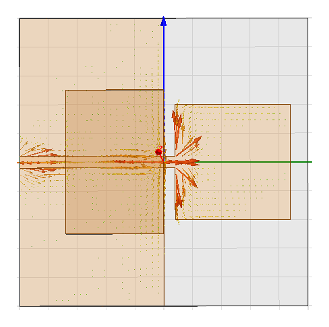
\includegraphics[width=0.3\linewidth]{Fig-aeue_4b.eps}}~~~
\subfigure[]{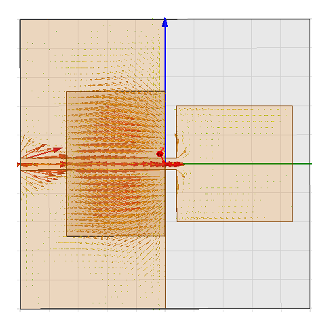
\includegraphics[width=0.3\linewidth]{Fig-aeue_4c.eps}}
\caption{(a) Current through $R_{Rad1}$ and $R_{Rad2}$ corresponding to the printed monopole antenna and the superstrate respectively. (b) Vector current density of the antenna at 2.4 GHz. (c) Vector current density of the antenna at 4.1 GHz.}\label{fig-ckt-current}
\end{figure}

It is observed that at 2.4 GHz, the current through $R_{Rad1}$, corresponding to the printed monopole antenna is high. The current through $R_{Rad2}$, corresponding to the superstrate is high near 4.5 GHz. However, at the resonant frequency of each section of the circuit, the current through the other part of the circuit also shows a local maximum point.

Here, the values of the circuit parameters obtained from the genetic algorithm are used for this analysis. The input resistance $R_{\text{in}}$ is fixed at 50 $\Omega$. This is the typical input impedance of an SMA connector, used for exciting a printed antenna. Both of the radiation resistances, $R_{Rad1}$ and $R_{Rad2}$ are fixed at 377 $\Omega$, which is the characteristic impedance of free space. Only the absolute value of the magnitude of the current is plotted.

The current density of the antenna obtained from full-wave simulation at 2.4 GHz and 4.1 GHz are shown in Figure \ref{fig-ckt-current} (b) and (c) respectively. It is observed that the current density is higher at the printed monopole antenna at 2.4 GHz and the current density is higher at the superstrate at 4.1 GHz. Thus, the equivalent circuit model perfectly explains the behavior of the antenna.

\section{Experimental Results and Discussions}\label{sec:expt_results}
This section covers the details of the experiments performed for determining the physical dimensions of the antenna and for evaluating its performance. These experiments include a parametric study of the antenna dimensions and evaluation of its resonant frequencies, gains, and radiation patterns through simulation and measurement.

\subsection{A Parametric Study of the Antenna Dimensions}
The physical dimensions of the antenna shown in Table \ref{table-dims} are tuned to study the influence of each dimension on the overall behavior of the antenna. Fig. \ref{fig-vars} shows the variation of the two resonant frequencies of the antenna with the length of the patch, $l_P$, the length of the superstrate, $l_S$, and the longitudinal spacing, $s$ between the superstrate and the patch. In each of the plots in Fig. \ref{fig-vars}, the other dimensions of the antenna are kept fixed as in Table \ref{table-dims}.

\begin{figure}[h]
\centering
\includegraphics[width=0.8\linewidth]{Fig-aeue_5.eps}
\caption{Variation of resonant frequency of the antenna with the (a) length of the patch, $L_P$, (b) length of the superstrate, $L_s$ (c) Spacing, $S$ between the superstrate and the patch.}\label{fig-vars}
\end{figure}

Fig. \ref{fig-vars} (a) shows that as the length of the patch increases, both the resonant frequencies of the antenna falls almost linearly. The length of the superstrate has a more impact on the second resonant frequency as a decreasing trend is observed from Fig. \ref{fig-vars} (b) for $l_S~>~17mm$. This observation clearly indicats the effect of the superstrate on the second resonant frequency of the antenna. The variation of the resonant frequencies of the antenna with $s$ is shown in Fig. \ref{fig-vars} (c). The desired resonant frequency and radiation pattern of the antenna are obtained for $s~=~2mm$.

\subsection{Return Loss Measurement}
\begin{figure}
\centering
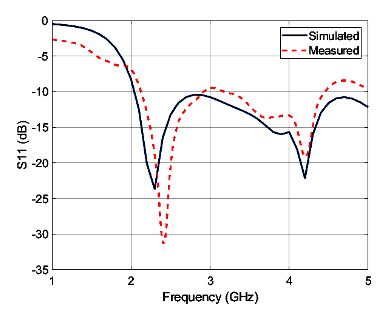
\includegraphics[width=0.5\linewidth]{Fig-aeue_6.eps}
\caption{The simulated and measured return loss (S11) parameter plot of the proposed antenna}\label{fig-s11}
\end{figure}

The simulated and the measured return loss (S11) parameter plot of the proposed antenna is shown in Fig. \ref{fig-s11}. The measurements are performed with a Rhode \& Schwarz ZNB-20 vector network analyzer (VNA). The antenna has two distinct wide operating bands. The first operating band covers the 2.4 GHz ISM band and the second resonant frequency covers the C-band of 5G wireless communication from 3.5 GHz to 4.2 GHz. The measurement result closely follows the simulation result with a minor deviation that may be attributed to an imperfection in the tolerance of fabrication.

\subsection{Radiation Pattern and Gain Measurement}
The co-polar and the cross-polar radiation patterns are measured for both the principal plane of the antenna at its peak resonant frequencies. The measurements are carried out with a standard horn antenna as the transmitter and the antenna under test on a turn table interfaced with the VNA. The measured radiation patterns are shown in Fig. \ref{fig-pat}. It is observed that the antenna provides an omnidirectional radiation pattern in the YZ-plane at 2.4 GHz and a directional radiation pattern in the YZ-plane at 4.2 GHz. The peak gains achieved at 2.4 GHz and 4.2 GHz are 3.1 dBi and 5.1 dBi respectively. All planes used for describing the radiation patterns are in accordance with the orientation of the antenna as shown in Fig. \ref{FabEqckt} (a).

\begin{figure}[h]
\centering
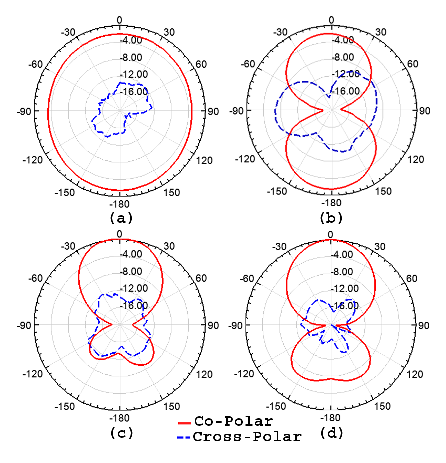
\includegraphics[width=0.5\linewidth]{Fig-aeue_7.eps}
\caption{Radiation pattern of the antenna in the (a) YZ Plane at 2.4 GHz (b) XZ Plane at 2.4 GHz, (c) YZ Plane at 4.2 GHz, (d) XZ Plane at 4.2 GHz}\label{fig-pat}
\end{figure}

\section{Discussions and Conclusion}\label{sec:concl}
From the analysis and the experimental results it is observed that the proposed antenna has two distinct far-field radiation patterns at its two resonant frequencies. An equivalent circuit model of the antenna is also proposed. The behavior of the antenna is explained with the equivalent circuit model. The parameters of the equivalent circuit model are obtained using vector-fitting technique and genetic algorithm. The accuracy of the equivalent circuit model is validated through comparison of its output current with the simulation results of the antenna.

The proposed antenna has an omnidirectional radiation pattern at the 2.4 GHz ISM band. At the C-band, the primary radiating element is the superstrate and the antenna has a directional radiation pattern with a higher gain due to the presence of the ground plane. At this band, the antenna is more suitable for directional communication. The antenna finds its possible applications in an IoT or WiFi network with a 5G backbone. 
\chapter{Synthesis of a Sparse 2D-Scanning Array using Particle Swarm Optimization for Side-Lobe Reduction}
\label{chap:chap5}
\section{Introduction}\label{c5sec_intro}
A phased array antenna is widely used in wireless communication and radar systems. With the evolution of 5G and millimeter-wave communication, a large grid of small printed antennas is becoming popular \cite{5gmmwave, 5gmmwave_fr4}.

A phased array antenna comprises stationary elements excited at different phases to obtain radiation in different directions \cite{phasedArrayHandbook}. Phased arrays have been there for a long time. The first phased array antenna was made in 1955 \cite{phasedArray_russia}. The first printed phased array was reported by Munson et al. in 1974 \cite{txmPhasedArray}. With the evolution of microwave and millimeter-wave communication standards, the use of phased arrays became more common. There has been extensive research on phased array antennas with a significant number of radiating elements for 5G wireless communication \cite{mmarrayRrev}.

The elements of a typical phased array have a spacing of one-half of the operating wavelength, represented by $\lambda/2$ \cite{phasedArrayHandbook}. A sparse array is a phased array antenna that has fewer elements than a conventional array. Synthesis of a sparse array reduces the overall cost, weight, required power, dissipated heat, etc. of a communication or a radar system because of the reduced number of elements of the array and the corresponding reduction in the excitation circuitry \cite{sparseDesignConstraints}.

When an array has a fewer number of elements, the spacing between the elements becomes greater than $\lambda/2$. This causes an increase in the number of side lobes of the antenna. This is a major drawback of sparse arrays. Traditionally, this problem was addressed by adjusting the positions, spacing, and excitation weights of the array \cite{sparseDesignConstraints}.

With the advancement of modern computers, soft-computational optimization algorithms are widely being used for the synthesis of sparse arrays. Synthesizing a sparse array from a fully populated array is called an array thinning problem. A solution to an array thinning problem using genetic algorithm was proposed by R. Jain et al. in 2012 \cite{thinningGA}. Another similar work was published by M. A. Zaman et al. in 2012 \cite{nunUniformLinear}. There are also analytical approaches for the synthesis of arrays. In 2016, E. Sandi et al. proposed a technique for the synthesis of sparse arrays using a combination of cyclic difference set and binomial amplitude tapering \cite{amplitudeTaperingHybrid}. Such approaches usually involve a complex mathematical formulation and limited usability.

In recent years, the synthesis of planar sparse arrays is emerging as a popular area of research. A modified genetic algorithm for the synthesis of planar arrays was proposed in 2017 by K. Y. Reddy et al \cite{randomlySpacedArray}. Another multi-objective optimization-based technique for sparse array synthesis was proposed in 2020 by H. Li et al \cite{selfOrgOpt}. In both of these works, the primary objective was to minimize the peak side-lobe power. The radiation pattern of the antenna is calculated numerically to obtain the value of the fitness function. There are also analytical approaches for the synthesis of planar phased array antennas. A singular value decomposition (SVD) based non-iterative approach for array synthesis was reported by P. F. Gu et al. in 2019 \cite{SyntLargeSparse}.

Arrays of printed antennas are most commonly used for millimeter-wave communication. Most of the printed antennas with a ground plane have a cosine radiation pattern. In this work, a sparse 2D phased array is presented with cosine antenna elements. The sparse array is synthesized from a $16\times 16$ uniform rectangular array (URA). The number of elements in the array is reduced by 50\%. The positions of the elements are tuned with Particle Swarm Optimization (PSO) algorithm to minimize the peak side-lobe level (PSLL).

The PSLL, gain and beam-width of the synthesized sparse planar array are compared with the original URA. It is observed that the synthesized sparse array yields a narrower beam-width than the original sparse array. A narrower beam-width is indicative of a better resolution of the scanning array \cite{sparseDesignConstraints}.

The remaining sections of the paper are arranged as follows. The design details of the $16\times16$ URA are presented in Section II. Section III covers the details of the synthesis and optimization of the sparse array followed by the experimental results and discussions in Section IV. The paper is concluded in Section V.

Matlab Phased Array System Toolbox$^{\circledR}$ is used for computing all radiation patterns used and presented in this work.

\section{DESIGN OF A $16\times16$ URA}\label{c5sec_design}
\subsection{Array Topology and Progressive Phase Excitation}
The topology of the uniform rectangular array is shown in Fig. \ref{fig_5_1}. It is a uniform array with a spacing of half of the wavelength ($\lambda/2$) in both directions. The antenna element used is a cosine element.

\begin{figure}
  \centering
  
\includegraphics[width=0.4\linewidth]{Fig-naun_1.eps}\\
  \caption{Topology of the URA} \label{fig_5_1}
\end{figure}

Along the direction of the azimuth plane, the $k^{th}$ element has a phase of $(k-1)\delta_{AZ}$. Similarly, the $m^{th}$ element along the direction of the elevation angle has a phase of $(m-1)\delta_{EL}$. Thus, the weight of excitation of the element $(k, m)$ in the 2D array is given by Eq. \ref{c5_eq1}.

\begin{equation}\label{c5_eq1}
\begin{split}
W & = e^{j(k-1)\delta_{AZ}} \times e^{j(m-1)\delta_{EL}}~=~e^{j[(k-1)\delta_{AZ} + (m-1)\delta_{EL}]} \\
  & = \cos[(k-1)\delta_{AZ} + (m-1)\delta_{EL}] + j\sin[(k-1)\delta_{AZ} + (m-1)\delta_{EL}]
\end{split}
\end{equation}

\begin{figure}
  \centering
  \subfigure[Progressive phase shift in the direction of azimuthal plane]{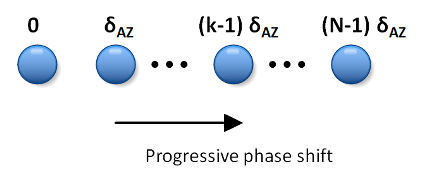
\includegraphics[width=0.4\linewidth]{Fig-naun_2a.eps}} ~~~~
  \subfigure[Progressive phase shift in the direction of azimuthal plane]{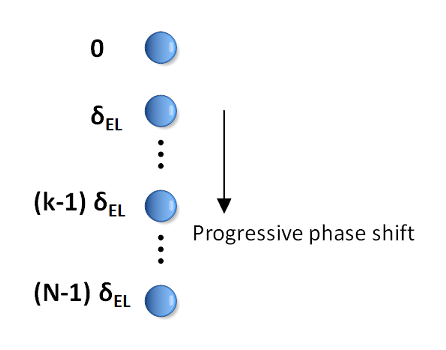
\includegraphics[width=0.4\linewidth]{Fig-naun_2b.eps}}\\
  \caption{Illustration of the progressive phase shift in excitation} \label{fig_5_2}
\end{figure}

The progressive phase shift is illustrated in Fig. \ref{fig_5_2}. For a uniform linear array, the analytical equations are available for estimating the values of the direction of the major lobe from the value of the progressive phase shift ($\delta$) \cite{phasedArrayHandbook}. In this work, an experimental method is used to understand this correlation for the 2D planar array. A dataset is created by varying both $\delta_{AZ}$ and $\delta_{EL}$ within a range of -135 degree to 135 degree at intervals of 15 degree resulting in a total of 361 scan-angles. The direction of the major lobe of the resultant radiation pattern is represented in terms of a combination of the azimuth angle ($\phi$) and the elevation angle ($\theta$) in a 3D polar coordinate system. The correlation plots are shown in Fig. \ref{fig_5_3}.

\begin{figure}
  \centering
  \subfigure[]{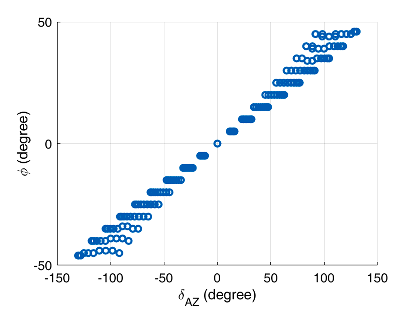
\includegraphics[width=0.4\linewidth]{Fig-naun_3a.eps}} ~~~
  \subfigure[]{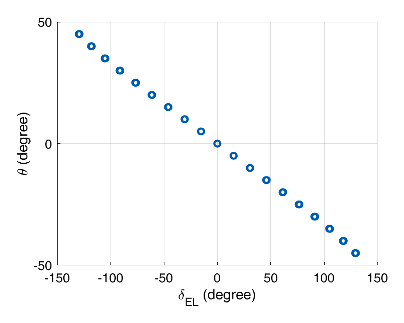
\includegraphics[width=0.4\linewidth]{Fig-naun_3b.eps}}\\
  \caption{Correlation of the (a) Azimuth angle ($\phi$) with $\delta_{AZ}$ and (b) Elevation angle ($\theta$) with $\delta_{EL}$} \label{fig_5_3}
\end{figure}

The sign of the correlation depends on the choice of the coordinate system. Here, the elevation angle is positive towards the top and negative towards the bottom and therefore a positive correlation is observed. The azimuth angle, on the other hand, is positive towards the right and negative towards the left leading to a negative correlation.

\subsection{Mapping the Radiation Angle to the Progressive Phase Shift using ANN}
From Fig. \ref{fig_5_3} (a) it is observed as $\delta_{AZ}$ and $\delta_{EL}$ is varied from -135 degree to +135 degree, the corresponding values of $\phi$ and $\theta$ vary from -45 degree to +45 degree. The elevation component of the radiation pattern shows a consistent linear correlation with the value of $\delta_{EL}$. However, the relation between $\theta$ and $\delta_{AZ}$ is not consistent. It is evident from this observation that the value of $\theta$ depends upon both $\delta_{AZ}$ and $\delta_{EL}$.

For modeling such systems, computational approaches are more suitable than analytical approaches since the computational models can detect hidden patterns in the data that cannot be observed or modeled analytically \cite{simDrivOptBook}. An artificial neural network (ANN) model is trained to map the angle of the major lobe ($\phi$, $\theta$) with the progressive phase angle ($\delta_{AZ}$, $\delta_{EL}$). The architecture of the ANN model is shown in Fig. \ref{fig_5_4}.

\begin{figure}
  \centering
  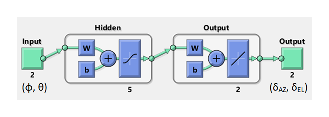
\includegraphics[width=0.6\linewidth]{Fig-naun_4.eps}\\
  \caption{Architecture of the ANN model to map the radiation angles ($\phi$, $\theta$) with the progressive phase angle ($\delta_{AZ}$, $\delta_{EL}$)} \label{fig_5_4}
\end{figure}

The ANN model is trained with the data set prepared for observing the correlation. Since the dataset is relatively small, a shallow network with 5 neurons in the hidden layer is selected for this purpose. The dataset is randomly split into test data and train data. The network is trained with a Bayesian Regularization algorithm which is suitable for smaller datasets \cite{bayesian_regularization, kumaresh_surrgoate}.

The error histogram of the neural network training is shown in Fig. \ref{fig_5_5}. A peak error of $\pm$1.15 degree is observed which is acceptable for this problem.

\begin{figure}
  \centering
  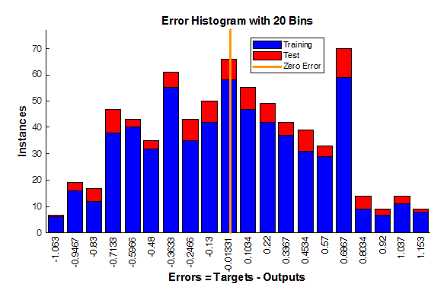
\includegraphics[width=0.5\linewidth]{Fig-naun_5.eps}\\
  \caption{Error histogram of the trained neural network} \label{fig_5_5}
\end{figure}

\section{Synthesis of Sparse Array}\label{c5sec_synth}
The key challenge in synthesizing a sparse scan-array is to ensure that the PSLL is minimized for all possible scan-angles or all possible combinations of $\delta_{AZ}$ and $\delta_{EL}$. Calculating the radiation pattern for all possible combinations is computationally very expensive. To make the experiment feasible, the radiation pattern is computed for three randomly selected ($\phi$, $\theta$) pairs. For each of these pairs, the corresponding values of $\delta_{AZ}$ and $\delta_{EL}$ are obtained from the trained ANN model. The radiation pattern of the antenna is computed for each of these three ($\phi$, $\theta$) pairs. The excitation weight matrix, W of the URA is calculated using Eq. \ref{c5_eq1}. The objective function returns the maximum PSLL value out of the three ($\phi$, $\theta$) pairs.

This step makes the objective function computationally expensive. To compensate for this, the PSO algorithm is used. The PSO is a widely used bio-inspired optimization algorithm and it is computationally less expensive than genetic algorithms (GA) as it requires fewer iterations \cite{pso_vs_ga}.

\begin{figure}
  \centering
  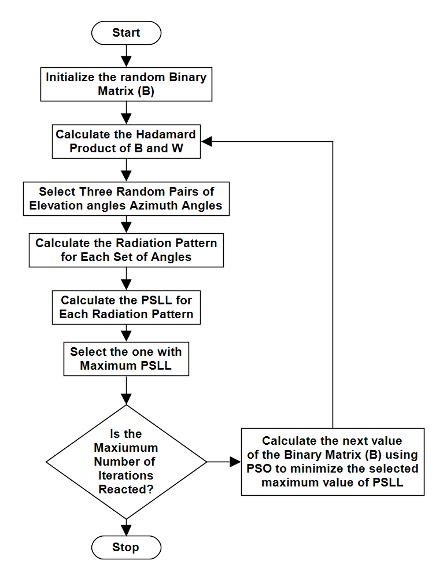
\includegraphics[width=0.5\linewidth]{Fig-naun_6.eps}\\
  \caption{Flow diagram of the sparse array synthesis steps using PSO} \label{fig_5_6}
\end{figure}

The flowchart of the proposed approach for sparse array synthesis using PSO is shown in Fig. \ref{fig_5_6}. Here, W is the excitation weight matrix of the $16\times 16$ URA. B is a binary matrix of size $16\times 16$. The weight of the sparse array is given by the Hadamard product of B and W ($B \odot W$). Thus, the optimization problem can be defined mathematically as:

\begin{equation} \label{eq_5_2}
Minimize~~F[B \odot W]
\end{equation}

Where F is the function that yields the maximum PSLL of the three randomly selected ($\phi$, $\theta$) pairs. In order to make sure that exactly 50\% of the elements are removed by the PSO, an additional constraint is added which is given by Eq. \ref{eq_5_3}.

\begin{equation}\label{eq_5_3}
\sum_{i,j}{\left[B_{i,j}\right]_{N\times N}} = \frac{N}{2}
\end{equation}

\section{Experimental Results and Discussion}\label{c5sec_res}
The $16\times 16$ URA is thinned into a sparse array using the method discussed in Section \ref{c5sec_synth}. In this section, the results of various experiments performed are covered to validate the accuracy of the proposed technique.

\subsection{The Architecture of the Sparsed Array}
The element positions of the synthesized sparse array are shown in Fig. \ref{fig_5_7}. Here, the number of elements in the sparse array is 128. The original $16\times 16$ URA has 256 elements. Thus, the number of elements in the array is reduced by 50\%.

\begin{figure}
  \centering
  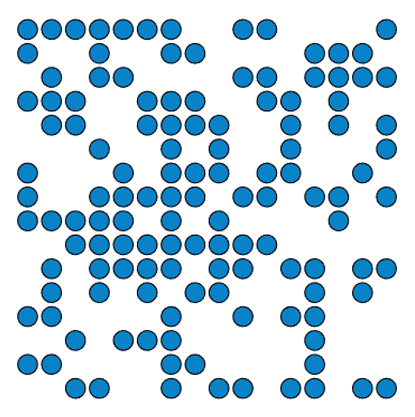
\includegraphics[width=0.4\linewidth]{Fig-naun_7.eps}\\
  \caption{Element positions of the synthesized sparse array.} \label{fig_5_7}
\end{figure}

It is observed that at some parts of the synthesized array, the vertical spacing of the original URA is maintained whereas, in some other parts, the horizontal spacing is maintained. This architecture guarantees that the excitation weights calculated for the URA work for the sparse array as well. Moreover, the elements that are scattered do not form any regular pattern. This suppresses the possibility of larger side-lobes that appear at multiples of the desired values of $\phi$ and $\theta$. It is difficult to obtain such solutions analytically.

\subsection{Analysis of the Direction of Main Lobe and PSLL}
The radiation patterns of the synthesized sparse array are analyzed for many combinations of the ($\phi$, $\theta$) pair. A part of these results is shown in Table \ref{tab_5_1}. The table shows the required values of $\phi$ and $\theta$, obtained values of $\phi$ and $\theta$, and the PSLL values of the URA and the sparse array.

\begin{table}[]
\caption{Some of the angles considered} \label{tab_5_1}
\centering
\resizebox{0.9\textwidth}{!}{%
\scriptsize
\begin{tabular}{|l|l|l|l|l|l|}
\hline
$\phi$ (deg) Desired & $\theta$  (deg) Desired & $\phi$ (deg) Obtained & $\theta$ (deg) Obtained & PSLL (dB) URA & PSLL (dB) Sparse \\ \hline
0 & 0 & 0 & 0 & -13.58 & -12.69 \\ \hline
0 & 45 & 0 & 45 & -11.64 & -11.59 \\ \hline
45 & 0 & 46 & 0 & -11.48 & -12.48 \\ \hline
45 & -45 & 45 & -45 & -10.38 & -9.89 \\ \hline
20 & 30 & 20 & 30 & -12.27 & -12.98 \\ \hline
-20 & 30 & -20 & 30 & -12.27 & -12.02 \\ \hline
-35 & -45 & -35 & -45 & -11.00 & -11.23 \\ \hline
10 & -45 & 10 & -45 & -11.60 & -11.73 \\ \hline
-10 & -40 & -10 & -40 & -11.85 & -11.75 \\ \hline
-30 & 40 & -30 & 40 & -11.58 & -11.98 \\ \hline
\end{tabular}%
}
\end{table}

It is observed that the values of $\phi$ and $\theta$ obtained are almost the same as the required values of the parameters. This observation validates the accuracy of the ANN model to predict the values of $\delta_{AZ}$ and $\delta_{EL}$. It also validates how the problem is formulated where the excitation weights of the sparse array are obtained from the Hadamard product of the weight matrix, W of the URA, and the binary matrix B.

The PSLL values are obtained from the normalized radiation pattern of the arrays. It is observed that the PSLL values of the sparse array are close to that of the original URA. Thus, there is no significant increase in the side-lobe level due to thinning the array. Fig. \ref{fig_5_8} shows the normalized radiation pattern of the antenna at $\phi$ = 30 degree and $\theta$ = 40 degree. For easier comparison, the values where the values of the radiation pattern are less than -- 60 dB are flattened.

\begin{figure}
  \centering
  \subfigure[]{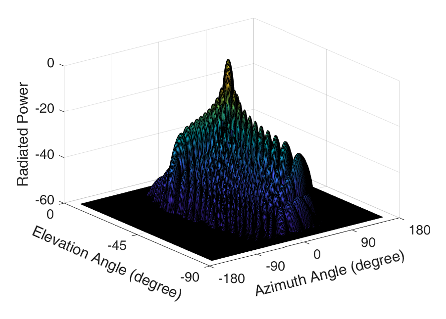
\includegraphics[width=0.4\linewidth]{Fig-naun_8a.eps}} ~~~~
  \subfigure[]{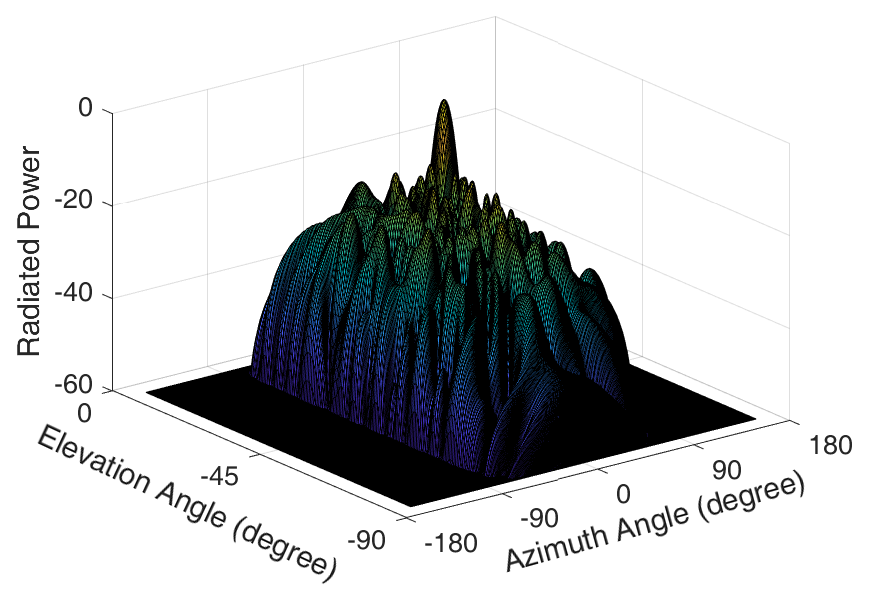
\includegraphics[width=0.4\linewidth]{Fig-naun_8b.eps}}\\
  \caption{The radiation pattern of the (a) URA and (b) the synthesized sparse array for $\phi$ = 30 degree and $\theta$ = 40 degree} \label{fig_5_8}
\end{figure}

From these figures, it is observed that the width and positions of the main lobe are identical for the URA and the sparse array. Although the sparse array has a larger number of side lobes, the values of these lobes are very small. Since the objective of the optimization problem was to suppress the PSLL only, the other side lobes are not significantly reduced.

It is not possible to include all the radiation patterns in this paper. Therefore, the overall PSLL values of the URA and the proposed sparse array are compared in a 3D surface plot shown in Fig. \ref{fig_5_9}. Here the values of $\phi$ and $\theta$ are tuned over the range of -- 45 degree to + 45 degree. It is observed that only at these two extreme points, the PSLL value of the sparse array is slightly higher than that of the original URA. As the $\phi$ and $\theta$ approach (0, 0), the values of the PSLL of the URA and sparse array become almost the same.

\begin{figure}
  \centering
  \subfigure[]{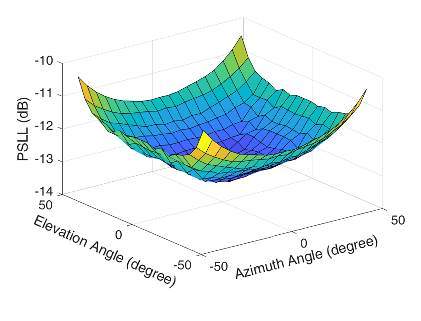
\includegraphics[width=0.4\linewidth]{Fig-naun_9a.eps}} ~~~~
  \subfigure[]{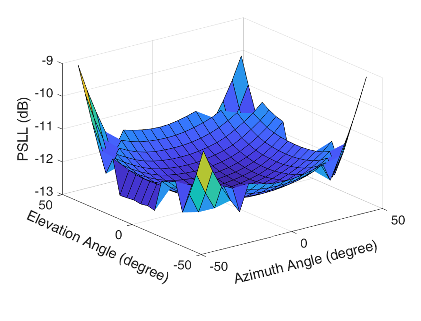
\includegraphics[width=0.4\linewidth]{Fig-naun_9b.eps}}\\
  \caption{Variation of PSLL with the direction of the main lobe for (a) URA (b) the sparse array} \label{fig_5_9}
\end{figure}

\subsection{Analysis of the Peak Gain}

As the number of elements is reduced to half, the peak gain of the antenna is also reduced. This section compares the gains of the original URA and the sparse array for all the possible angles of the elevation plane and the azimuthal plane ranging from -- 45 degree to 45 degree. From Fig. \ref{fig_5_10}, it is observed that as the distribution of the gains with the angle of the main lobe shows a similar trend for both the original URA and the sparse array. The difference in gain is maximum at the edges and reduces as the azimuth and elevation angles are close to zero. The difference in gain observed is 2 dB whereas the maximum difference is 4.5 dB.

\begin{figure}
  \centering
  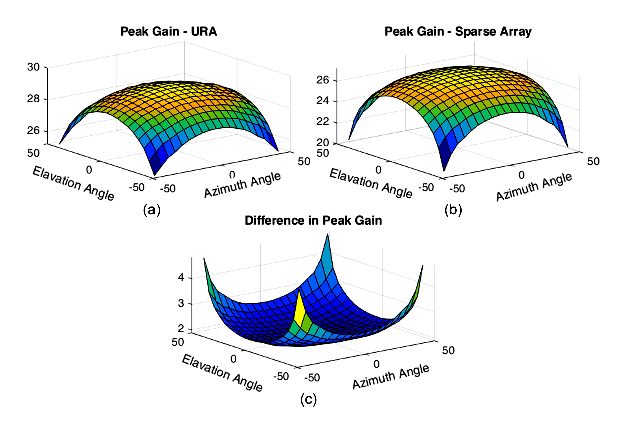
\includegraphics[width=0.95\linewidth]{Fig-naun_10.eps}\\
  \caption{(a) Distribution of the peak gain of the URA, (b) Distribution of the peak gain of the sparse array, (c) Difference between peak gains of URA and Sparse array} \label{fig_5_10}
\end{figure}

\subsection{Analysis of the Beam-width}
The beam-width is another important factor to be considered when a sparse array is synthesized. The beam-width and PSLL are often considered related constraints in many applications \cite{arrayTradeoffs}. The beam-widths of the original URA and the synthesized sparse scan-array are plotted for azimuth angles and elevation angles in the range from -- 45 degree to 45 degree in Fig. \ref{fig_5_11}.

\begin{figure}
  \centering
  \includegraphics[width=0.95\linewidth]{Fig-naun_11.eps}\\
  \caption{Distribution of the beam-width for (a) the original URA and (b) the synthesized sparse array} \label{fig_5_11}
\end{figure}

\begin{figure}
  \centering
  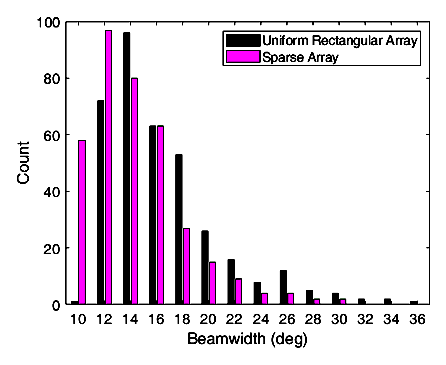
\includegraphics[width=0.5\linewidth]{Fig-naun_12.eps}\\
  \caption{Histogram of the beam widths of the URA and the sparse planar array.} \label{fig_5_12}
\end{figure}

From Fig. \ref{fig_5_11} (a) and (b) it is observed that the beam-width of the two arrays exhibit almost similar variations with the scan-angles. The maximum beam-width of the URA is 36 degree whereas that of the sparse array is 29 degree. The histogram of the beam-widths of the two arrays is shown in Fig. \ref{fig_5_12}. The sparse array has more scan-angles where the beam width is between 10-12 degrees. Beyond the beam-width of 16 degree, the number of points is lower in case of the sparse array as compared to the URA. It infers that the sparse array has narrower beam-widths than the URA.

\section{Conclusion}
A technique for synthesizing a sparse array from a $16\times 16$ URA is presented. The excitation weight matrix, W of the URA are estimated using an ANN model from the desired scan-angle. The PSO is used for obtaining a binary matrix B, such that the Hadamard product of B and W yields the excitation weights of the sparse antenna array. The experimental results show that the desired scan-angles of the sparse array are accurately obtained using this technique.

The PSLL of the URA and the sparse array are compared for all possible scan-angles in a range of -- 45 degree to + 45 degree for both the elevation plane and the azimuthal plane. It is observed that the PSLL of the synthesized sparse array is almost the same as that of the URA except at the extreme ends of the scanning range.

The overall scan angle of the proposed antenna array is 90 degree for both the azimuth plane and the elevation plane. The array comprises cosine antenna elements that represent printed antennas used in 5G millimeter-wave wireless communication. A comparative analysis of the original URA and the sparse array is observed in terms of gain and beam-width. It is observed that although there is a slight reduction in the gain of the sparse array, the beam-width is less indicating a better resolution for radar or directional wireless communication.

\chapter{Conclusion and Future Direction}
\label{chap:chap6}
%\minitoc
This chapter summarizes the overall findings and the outcomes derived out of the work. The chapter also highlights some of the possible future directions that may extend the work.

\section{Chapter Wise Findings}
The design and optimization of printed antennas is a vast domain of research. There have been research works worldwide in various areas of the domain. The present work primarily focuses on three  aspects of the domain. The findings of each domain are summarized as follows.
\begin{itemize}
\item \textbf{Optimization of Printed Antennas}: In \emph{Chapter \ref{chap:chap3}}, the optimization of the physical dimensions of a printed slot antenna is presented. Here, the primary contribution is the implementation of genetic algorithm within the script interface of a commercially available full-wave electromagnetic solver. The proposed approach significantly reduces the computational cost of optimizing printed antennas using a soft-computational optimization algorithm.

    The approach is used for optimizing the feeding position of the printed slot antenna. The performance of the antenna is validated form simulation and measurement results. Since a full-wave solver is used to compute the cost function of the optimization process, the performance of the optimized antenna agrees closely with measurement results.

\item \textbf{Analytical Modeling of Printed Antennas}: \emph{Chapter \ref{chap:chap4}} includes the design of a dual band antenna. The antenna has a omnidirectional radiation pattern at the 2.4 GHz ISM band whereas a directional radiation pattern at the C-band of sub 6 GHz 5G wireless communication.

    The proposed antenna is a hybrid of a printed monopole antenna excited by a microstrip line feed and a microstrip patch antenna excited by proximity coupled microstrip antenna. An equivalent circuit model of them proposed antenna is derived to explain the working of the antenna. The equivalent circuit model has two RLC networks corresponding to the two parts of the antenna each of which is responsible for a resonant frequency. The values of the lumped elements of the equivalent circuit model are estimated using GA. It is shown that the derived equivalent circuit model is able to mimic the current distribution of the antenna at different parts of the antenna at its resonant frequencies. It may be concluded that an analytical model of an antenna derived using soft-computational techniques are capable of explaining an antenna closely.

\item \textbf{Computer Aided Design of Printed Antenna Array}: The design of a printed array is presented in \emph{Chapter \ref{chap:chap5}}. In this work, a $16\times 16$ rectangular array is thinned to minimize the peak side lobe level (PSLL). The number of elements of the array is reduced by 50\% using PSO to minimize the SLL for the entire range of scan angles.

    The proposed sparse array has a scanning range of $\pm$45 degree in both azimuth and elevation plane. The objective function is defined in a way to minimize the PSLL of the sparse array for the main lobe in multiple possible directions in this range. The gain and bandwidth of the sparse array is almost the same as the original URA.
\end{itemize}

\section{Limitations}
The primary limitations of the present works are as follows:
\begin{itemize}
\item In the first work, only the feeding position of the printed slot antenna is optimized using genetic algorithm implemented using the script interface of AEDT. Since AEDT is a frequency domain finite elements solver, the time required for computing a single iteration of the optimization process is high. As a result, the computation time increases exponentially with the number of dimensions to be optimized. The optimization of multiple physical dimensions of the antenna may take a long time using this approach.
\item The second work presents the derivation of the equivalent circuit model of a dual-band antenna. The proposed equivalent circuit can explain the working of the antenna. However, the calculated values of the lumped elements of the equivalent circuit model corresponds to a fixed set of physical dimensions of the antenna. No mathematical relation between the physical dimensions of the antenna and the lumped circuit parameters could be established. As a result, this circuit may not be suitable for application as a physics based surrogate model to optimize an antenna.
\item The performance of the sparse array synthesized in the third work is validated through the phased array toolbox of Matlab. Because of the large size of the array and its inherent design complexities, the antenna could not be manufactured. The performance of the antenna could not be validated from measurement results. Without the measurement results, the applicability of the antenna in a real-world situation could not be ascertained.
\end{itemize}

\section{Conclusion}
The application of soft-computational optimization algorithms are explored in three different areas of printed antenna and array design. These approaches include the optimization of the physical dimensions of an antenna, obtaining the physical dimensions of an antenna, and the optimization of a printed antenna array. Each work is supported by experimental results and discussions. In the first work, an implementation of the genetic algorithm within a commercially available full-wave solver for optimization of the physical dimensions is presented. The second work covers the synthesis of an equivalent circuit model of a dual-band antenna using particle sward optimization algorithm. The resonant frequency and the current distribution of the antenna are predicted with the equivalent circuit model with high accuracy. The third work includes the synthesis of a sparse planar array from a uniform rectangular array.

From these works, it is observed that the soft-computational optimization algorithms may be applied to solve a variety of problems in the domain of printed antenna and array design. Different problems require different approaches for fitting these algorithms in the most suitable manner. Although there have been a significant amount of research in the recent years in this direction, there are still many unexplored areas that require further investigation.

\section{Future Direction}
The design and optimization of printed antennas and arrays is an active area of research. The present work touches three of the most significant areas of research in the domain of antenna research. The work on each of these areas may be extended further in order to design something that may be readily deployed for real world applications. Some of the possible future directions extending the current work are as follows.
\begin{itemize}
\item Genetic Algorithm is implemented in the Python script interface of AEDT to optimize a printed antenna as discussed in \emph{Chapter \ref{chap:chap3}}. More optimization algorithms such as particle swarm optimization, differential evolution, etc. may be implemented in a similar approach as there are use cases where these algorithms yield better optimization performance in comparison to genetic algorithm.
\item The proposed computer aided equivalent circuit model of a multi-layer antenna, discussed in \emph{Chapter \ref{chap:chap4}}, may be used as a physics-based surrogate model to optimize the physical dimensions of the antenna to improve its performance in terms of gain, bandwidth, resonant frequency, etc. Physics based surrogate models are low-fidelity models that may be computed faster at a much less computing cost. The design time of the antenna is significantly reduced when surrogate models are used to compute the cost function.
\item In  \emph{Chapter \ref{chap:chap5}}, the design of a printed sparse array is presented. Because of the large size of the antenna, it could not be fabricated and the performance of the array could not be evaluated from measurement results. Fabrication of such large planar arrays is a challenge in itself. There is a scope of further research in finding a cost-effective and efficient approach for fabricating such array along with the feeding mechanism. 
\end{itemize} 
%=====================================================================

%=====================================================================
% BIBLIOGRAPHY
%   This should follow the appendices, if any, otherwise summary and
%   conclusions chapter.
% Choose your bibliography style
% plain is the basic style, others include ieeetr, siam, asm, etc
\bibliographystyle{ieeetr}
\bibliography{references}
%\begin{itemize}
%\item \textbf{PAPER PUBLISHED AND ACCEPTED:}\\
%\begin{enumerate}
%\item
%\item
%\end{enumerate}
\chapter*{Publications}
\addcontentsline{toc}{chapter}{Publications}
\section*{Paper Accepted/Published in International Journal:}
\begin{enumerate}
\item S. Goswami, K. Sarmah, P. Borah, and K. K. Sarma, ``Design of a dual-band multilayer antenna and its equivalent circuit modeling with vector-fitting and genetic algorithm,'' \emph{AEUE - International Journal of Electronics and Communications}, vol. 138, p. 153838, Aug. 2021, doi: 10.1016/j.aeue.2021.153838.
\item S. Goswami, K. Sarmah, K. K. Sarma, and N. E. Mastorakis, ``Synthesis of a Sparse Planar Phased Array Antenna with Reduced Side-Lobe Level and Beam-Width using Particle Swarm Optimization,'' \emph{International Journal of Circuits, Systems and Signal Processing}, vol. 15, pp. 1387-1393, Sep. 2021, doi: 10.46300/9106.2021.15.148.
\item S. Goswami, K. Sarmah, and K. K. Sarma, ``Analytical Methods Revisited: A Search for Possible Candidates for Physics Based Low-Fidelity Models of Patch Antennas,'' \emph{Indian Journal of Physics}, 2022. (Published online on March 25, 2022). doi: https://doi.org/10.1007/s12648-022-02319-x
\end{enumerate}

\section*{Book Chapter Published:}
\begin{enumerate}
\item S. Goswami, K. Sarmah, and K. K. Sarma, ``Simulation-Driven Optimization of Slot Antenna Using Genetic Algorithm,'' in \emph{Planar Antenna - Design, Fabrication, Testing, and Application}, Nova Science Publishers, Inc., USA, 2021.
\end{enumerate}

\section*{Paper Published in International Conference:}
\begin{enumerate}
\item S. Goswami, K. Sarmah, K. K. Sarma, and N. E. Mastorakis, ``Synthesis of a Sparse 2D-Scanning Array using Particle Swarm Optimization for Side-Lobe Reduction,'' in proc. \emph{24th International Conference on Circuits, Systems, Communications and Computers}, Crete Island, Greece, July, 2021.

    (Published in WSEAS Transactions on Communications, vol. 20, p. 112-116, 2021, doi: 10.37394/23204.2021.20.14)
\end{enumerate} 
\end{document}
